\small
\renewcommand{\thefigure}{A\arabic{figure}}
\setcounter{figure}{0}

This part holds every result removed from the main text, with every number unchanged. Verdict words are the registered ones. Appendix~\ref{app:K} holds the oracle arm and the \pizero{} replication, which Sections~\ref{sec:grid} and~\ref{sec:pi0} summarise, and Appendix~\ref{app:L} holds the paragraphs and tables that the trim of the main text removed.

%=====================================================================
\section{Setting details}
\label{app:A}

\textbf{Models.} \pifive{} (openpi pi05\_libero), \pizero{} (pi0\_libero), GR00T N1 (groot\_libero), X-VLA (xvla-libero), SmolVLA (smolvla\_libero). X-VLA enters the atlas and the F7 reads and misses the transport reads, because its server sends absolute end-effector targets and our ReGuide transports issue delta commands.

\textbf{Scenes.} Scene 1 has 11 tasks: K1--K4 and K6, and N1--N6 (cheese or wine bottle with plate, stove, cabinet or bowl). It has two layouts, one with the trained start regions and one that shifts them. Scene 2 is LIBERO-10's LIVING\_ROOM\_SCENE5 (white mug, yellow-and-white mug, red mug, left plate, right plate); its trained task puts the white mug on the left plate and the yellow-and-white mug on the right plate. In scene 2, K1 and K2 are the two halves of the compound, and N1 and N2 re-pair the mugs and plates. The testability floor says a model is testable on a scene only if it scores at least .70 on the trained tasks; scene-2 GR00T scores .508 [.333, .667].

\textbf{States.} Scene 1 uses 20 development states, 20 further states and blocks of 40 to 60 states. Scene 2 uses 60.

\textbf{Reference planner.} U scores .894 on held-out pairings of scene 1 from simulator poses, .883 from camera poses and .881 from a learned segmenter. In scene 2 it scores .967 on N2 and .333 on N1, pooling to .65 [.25, 1.00].

\textbf{Criteria for architecture-rooted failures.} C1: the input holds the needed information and the reference planner reaches .80. C2: the failure persists across models (models, chunk length, prompting; no data ladder). C3: a structural change that adds no information removes the failure. A failure that misses C1 belongs to the task. We phrase C3 as ``adds no task information beyond a calibrated RGB-D sensor''.

\textbf{Registration.} Each confirmatory read has a pre-registered record written before any main rollout. Verdicts appear in capitals (SUPPORTED, NOT SUPPORTED, NOT SHOWN, REVERSED, PARTIAL, EQUIVALENT, NON-INFERIOR, UNTESTABLE).

\textbf{Frame rule.} Every episode drawn in Figures~\ref{fig:teaser} and~\ref{fig:gallery} and in the frame figures of this appendix (Figures~\ref{fig:A2}--\ref{fig:A9}, \ref{fig:A16} and~\ref{fig:A14}) is a development-state episode, and the rule that picks it was fixed before any frame was looked at. Per entry, over its first 10 trials in a fixed order, a trial qualifies if the failing arm fails with the failure's own signature and the comparator arm succeeds on the same trial of the same run. The shown episode is the lowest-index qualifying trial, and Figure~\ref{fig:A16} shows the next three. If no trial of the first 10 qualifies, 10 more trials run and the same rule applies. The episodes are not a sample: they are chosen by outcome, and the registered rate in each caption is the cell's rate over all its states. The F6 signature was revised once, after the failure-mode classification of Appendix~\ref{app:B} and before the selection was recomputed (from ``released more than 3 cm away'' to ``failed and the final bowl xy more than 3 cm from the plate centre''; the original version flagged 6 of 50 \pifive{} F6\_b failures). Frames come from new rollouts that log their own outcome, so a re-run of a registered state can differ from its registered result.

\begin{figure}[t]
\centering
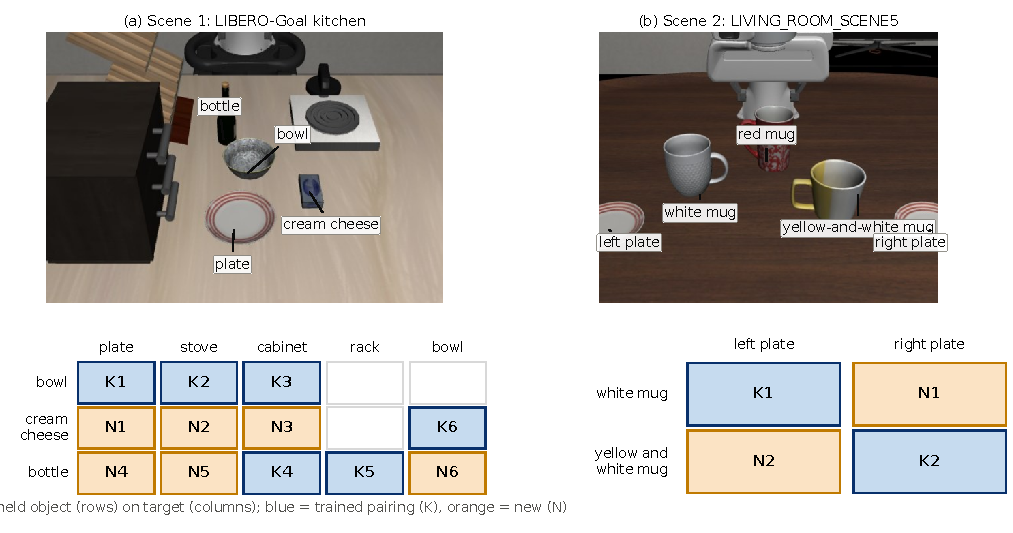
\includegraphics[width=\textwidth]{figA1.pdf}
\caption{Scenes and task set. Scene 1 (LIBERO-Goal kitchen) and scene 2 (LIVING\_ROOM\_SCENE5) as simulator renders with labelled entities, and, below each render, its pairing grid (scene 1: held object by target, K1--K6 trained pairings and N1--N6 new pairings; scene 2: mug by plate, K1, K2 trained and N1, N2 new), with trained cells in blue and new cells in orange. The renders are start states, not rollouts.}
\label{fig:A1}
\end{figure}

%=====================================================================
\section{The failure atlas in detail}
\label{app:B}

\begin{figure}[t]
\centering
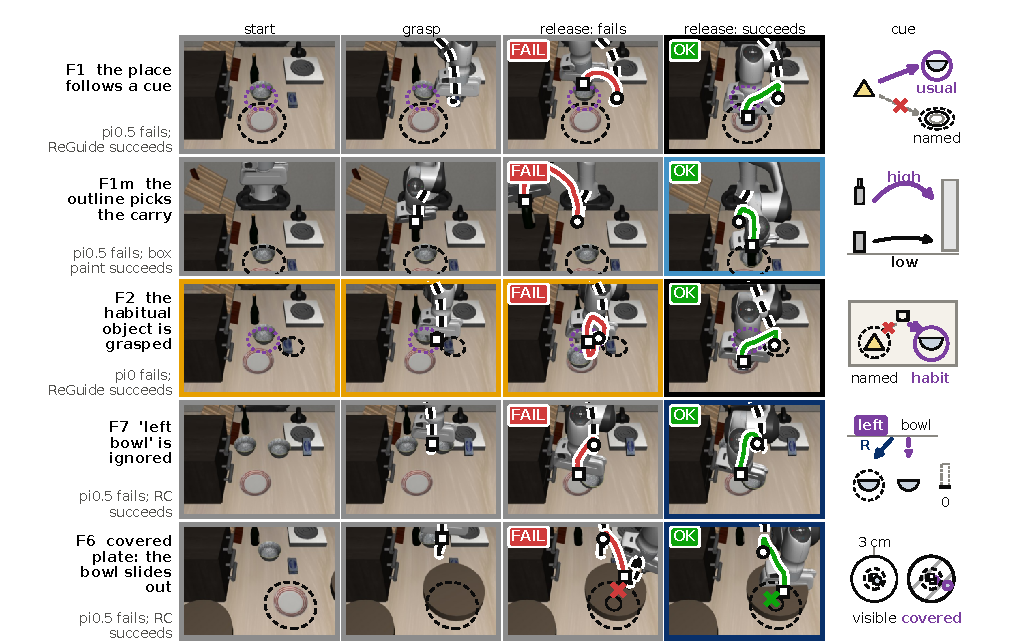
\includegraphics[width=\textwidth]{fig_gallery.pdf}
\caption{The failures in frames, scene 1: start, grasp and release of the failing arm (FAIL), release of the comparator on the same trial (OK), and the cue schematic. Registered rates: F1 E +.450 [.28, .61]; F1m N4+N6 .625 against .812 with the bottle painted as its box; F2 grasp excess +.650 [.39, .88] on \pizero{} and +.833 [.67, .96] on SmolVLA; F7 .40 (SP) and .20 (NG) for \pifive{} against 1.00 and .775 with the resolver; F6 cost of covering .38 [.28, .48]. Development-state episodes chosen by outcome (Appendix~\ref{app:A}); scene 2 is in Figure~\ref{fig:A3}.}
\label{fig:gallery}
\end{figure}

\begin{table}[h]
\caption{Measured break by failure and model. E is the excess failure over known partners.}
\label{tab:B1}
\centering
\footnotesize
\setlength{\tabcolsep}{3pt}
\begin{tabularx}{\textwidth}{@{}>{\raggedright\arraybackslash}p{1.15in}XXXXX@{}}
\toprule
failure & \pifive & \pizero & GR00T N1 & X-VLA & SmolVLA \\
\midrule
F1, scene 1, cross-chunk E, held-out states & +.450 [.28, .61] & +.225 [.05, .43] & +.500 [.26, .74] & +.379 [.04, .73] & +.054 [\mi.00, .14], no break \\
F1, scene 2, cross-chunk E & +1.000 [1.00, 1.00] & +.908 [.792, 1.00] & +.533 [.167, .858], below floor & & \\
F1m, N4 and N6 & succeeds .04 after a high carry, .66 after a low one & high carry on .67--1.00 of grasps & high carry on at least .78 & high carry on 1.00 & \\
F2, grasp E, held-out states & +.000 [.00, .00] & +.650 [.39, .88] & +.017 [.00, .07] & +.192 [.00, .53] & +.833 [.67, .96] \\
F7, relational choice equals ambiguous choice & .925 (SP), 1.00 (NG) & ignored on 4 of 6 cells across \pizero, X-VLA, SmolVLA, agreement 75--100\% & 1.00 (SP), 1.00 (NG, PARTIAL) & see \pizero & see \pizero \\
F6, cost of covering the plate, d \mi{} b & .38 [.28, .48] & not testable, gate .017 & .60 [.51, .68] & & \\
New layout & NEITHER & NEITHER & NEITHER & NEITHER & NEITHER \\
\bottomrule
\end{tabularx}
\end{table}

\begin{figure}[t]
\centering
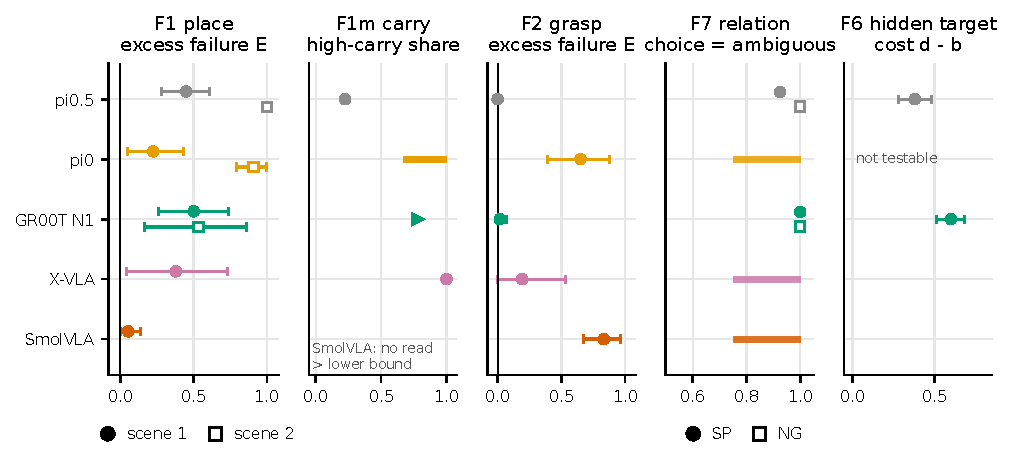
\includegraphics[width=\textwidth]{fig_atlas.pdf}
\caption{The measured break of each failure on the five frozen VLAs (a blank row means no read): excess failure E over known partners with 95\% intervals (F1, F2; F1 scene 1 filled, scene 2 open), share of grasped N4 and N6 episodes that start the high carry (F1m), share of states where the relational choice equals the ambiguous choice (F7), and cost of covering the plate, d \mi{} b (F6; \pizero{} not testable). Frozen \pifive{} is grey. Numbers are those of Table~\ref{tab:B1}.}
\label{fig:atlas}
\end{figure}

\textbf{F1.} Trained tasks run at .98--1.00 on \pifive{} and GR00T in scene 1. SmolVLA fails inside the chunk (within-chunk E +.862 [.73, .96]). The four cross-chunk verdicts replicate from development to held-out states. In scene 2 every model scores 0 of 720 on the two held-out pairings while \pifive{} scores .99 and \pizero{} .81 on the trained halves; the swapped two-step task scores 0 of 180 and ends in the trained arrangement on .83--.98. Chunk lengths of 2 and 10 change \pifive{} by \mi.050 [\mi.250, +.150] and \mi.042 [\mi.200, +.100] and GR00T by \mi.008 [\mi.117, +.100] and +.083 [\mi.025, +.233]. The scene-2 cue series on \pifive: with the mugs' start positions swapped, 287 of 287 placements go to the start-side plate; \pizero{} gives .993 of 145; with the plates moved, 0 of 116 and 0 of 125 disagreeing placements go to the start-side plate; with the nearer plate the less salient one, 158 of 158 placements go to the small nearer plate when it is the trained one, and .859 of 149 to the large far plate when that is the trained one. Majority rule: trained plate outvoted 153 of 153, salient plate .974 of 151, nearer plate .752 [.660, .843] of 141; earlier layouts replicate at .970 of 427. The planner meets C1 on three layouts (.825--.838) and misses it on three (.725--.788). Fixes: the front end tvpb lifts \pifive{} from .454 to .938 with no trained-task cost. The hand-over to a parts policy lifts GR00T from .17 to .84 and \pifive{} from .50 to .85 [+.017, +.675] (NOT SHOWN for \pifive). In scene 2 a reimplemented ReGuide lifts \pifive{} to .708 [.650, .775] on N1+N2 and \pizero{} to .700. The majority rule holds on \pifive{} only; \pizero's labels are unresolved on two layouts, and GR00T matches nearer-plate routing below its floor. \citet{grant2603} hold the attention-path probe.

\textbf{F1m.} The planner P\_min scores .80 on N4 and .80 on N6. From a pre-grasped pose 6 cm above the target the servo scores 25 of 26 and a bare release 21 of 26; with the bottle held above the target \pifive{} places 26 of 26. Painting the held bottle as its box lowers the high-carry share from .225 to .062 and raises N4+N6 from .625 to .812 (+.188 [+.075, +.325]) with no known-task cost. On GR00T the same box adds +.025 [\mi.025, +.100] (UNRESOLVED) at \mi.070 on trained tasks. ReGuide's transport takes GR00T's N4 high-carry share from 1.00 to 0 of 38; N6 still carries high on .821 and reaches .200. GR00T's N6 places 0 of 14 even from above the bowl. The cue is the outline on \pifive{} and does not transfer.

\textbf{F2.} Frozen \pifive{} and GR00T grasp the named object at .950--.992. On \pizero{} and SmolVLA .679 and .829 of held-out episodes end at the grasp. In scene 2, \pifive{} puts back a held mug the instruction does not name and grasps it again 240 of 240 times; after a clear-away carry it takes the named mug on .167 of N2 episodes and after its trained white-mug carry on .967. ReGuide's approach transport lifts \pizero{} from .021 to .608 and SmolVLA from .021 to .604, with trained tasks at +.020 [.000, +.060] and +.030 [\mi.020, +.120]; in scene 2 it moves \pifive's first hold to the named mug on 60 of 60 N2 episodes against 0 for the hand-over alone. Role views alone lift \pizero{} by +.183 [+.021, +.412] and do nothing on SmolVLA.

\textbf{F7.} With two identical bowls, only the relation picks the referent. With the other bowl removed the models score .825--1.00 and the scripted references .93--1.00. Referent share is .475--.50. On \pizero, X-VLA and SmolVLA the relation is ignored on 4 of 6 cells; X-VLA and SmolVLA on SP have no power; F7 holds on all five VLAs on at least one family. A negated LIBERO-PRO instruction scores 0 of 20 on \pifive{} and GR00T against .95 for the trained one (descriptive). A resolver plus a role view paints the other bowl: it fixes 3 of 4 cells with the resolver exact on 160 of 160; \pifive{} goes from .40 to 1.00 (SP) and .20 to .775 (NG), GR00T SP from .30 to .85. On \pizero, X-VLA and SmolVLA it fixes 0 of 6 cells (resolver exact 240 of 240), because those models fail even the named plate bowl on 0 of 20. GR00T's NG cell is capped at .50 by its unique-name control. \citet{wulff2610} report that \pifive{} and GR00T N1.7 respond most to empty and directional instructions, with the strongest directional effect in GR00T's early layers; they measure the change in flow-matching loss under patching on LIBERO-10 demonstration steps and do not measure task success or the action chunk, whereas we measure the chunk change of \pifive{} under a left-right swap (.004 in Appendix~\ref{app:D}), so the two results use different perturbations and different measures.

\textbf{F6.} The plate appears displaced and a cylinder then covers it (a never, b after the first query, c from the start, d beside the plate). The planner reaches .839 on 120 states; d keeps \pifive{} at .967 and GR00T at .742. Covering costs \pifive{} .38 [.28, .48] and GR00T .60 [.51, .68]; b stays within .05 of c (+.05 [\mi.05, +.158] and +.042 [\mi.033, +.117]); PARTIAL on both models (equivalence bound missed by .058 and .017). A memory overlay raises \pifive{} from .58 to .84 (+.26 [+.15, +.35]) and GR00T from .14 to .28 (+.14 [+.04, +.24]). Failure-mode classification (opaque cylinder with collisions off; LIBERO's On(): bowl centre within 3 cm xy and in contact): of 50 failures of frozen \pifive{} under b (success .583, 120 states), 44 release within 3 cm of the centre (median 1.8 cm) and 6 release 3--10 cm away; the bowl slides about 2.6 cm and ends 4.05 cm from the centre against 2.07 for successes. c gives .533, about b; a gives .942, d .967, the overlay .842. GR00T's b failures release 3 cm or more away on 76\%, ending about 21 cm away. The plate leaks into view on 32--49\% of later queries; GR00T sits at the rule's boundary and the overlay trails d by \mi.458 [\mi.558, \mi.358]; \pizero{} is not testable (gate .017).

\textbf{New layout.} Success on N1--N6 is .30 on \pifive{} and .08 on GR00T; the scripted servo scores .31, P\_min .37 and U .378; all fail on the same states; the demo's fixed top-down grasp holds on 0 of 10 cheese and 0 of 10 bottle states. C1 fails, so this is a limit of the task.

\textbf{Fixes by group.} Input-only: role views plus phrases lift \pifive{} .450 to .817 (+.367 [+.092, +.634]) with trained tasks \mi.010 [\mi.08, +.04]; silhouettes beat a grey proxy by +.442 [+.208, +.675]; phrases alone add +.025 [\mi.15, +.19]; tvpb reaches .938 against .454; on GR00T views add +.186 [+.033, +.361]. In scene 2 views give .000 on \pifive{} and GR00T; before a hand-over they lift N1+N2 to .508 at \mi.108 [\mi.158, \mi.058] on trained tasks. On \pizero{} and SmolVLA tvpb costs trained tasks \mi.485 [\mi.725, \mi.220] and \mi.935 [\mi1.00, \mi.810]. Transport-level (ReGuide reimplementation): \pifive{} .929 against tvpb .938 (+.008 [\mi.083, +.092], EQUIVALENT); GR00T N1--N6 .212 to .838 (+.625 [+.350, +.879]); scene 2 N1+N2 .708 on \pifive{} and .700 on \pizero, beating our hand-over by +.350 [+.242, +.458]; without rendered depth .700 [.633, .775] on \pifive{} and .608 on \pizero. Our hand-over reaches .442 (simulator) and .450 (perception). Resolver and memory composite RC: beats ReGuide alone on F7 by +.550 [+.488, +.625] (SP) and +.663 [+.587, +.738] (NG) with trained tasks \mi.008 [\mi.025, .000]; on F6 the slot lifts \pifive{} from .517 to .817 (+.300 [+.167, +.433]); RC beats ReGuide by +.167 [+.050, +.284]; ReGuide's pose registration shows no measured memory (+.117 [\mi.033, +.267]); on \pizero{} the composite beats ReGuide on SP by +.375 and costs K1t \mi.100 [\mi.183, \mi.033] (PARTIAL).

\textbf{N1 residual in scene 2.} N1 stays at .417--.500 under perceived poses and reaches .833--.900 under simulator poses. The rigid held-mug estimate sits 5.65 cm off at release; a box tracker leaves it at 5.71 cm (N1 +.133 [\mi.033, +.283], NO CLEAR DIFFERENCE; N2 fell by .583). Swapping the simulator's held-mug pose gives .567 against .500 (+.067 [\mi.067, +.200]), the target-plate pose .450 (\mi.050 [\mi.183, +.084]); the oracle variant reaches .900, +.333 [+.183, +.467] over the held-mug swap, which also switches the interaction rule. The reading of the hold and release events is untested.

\begin{figure}[t]
\centering
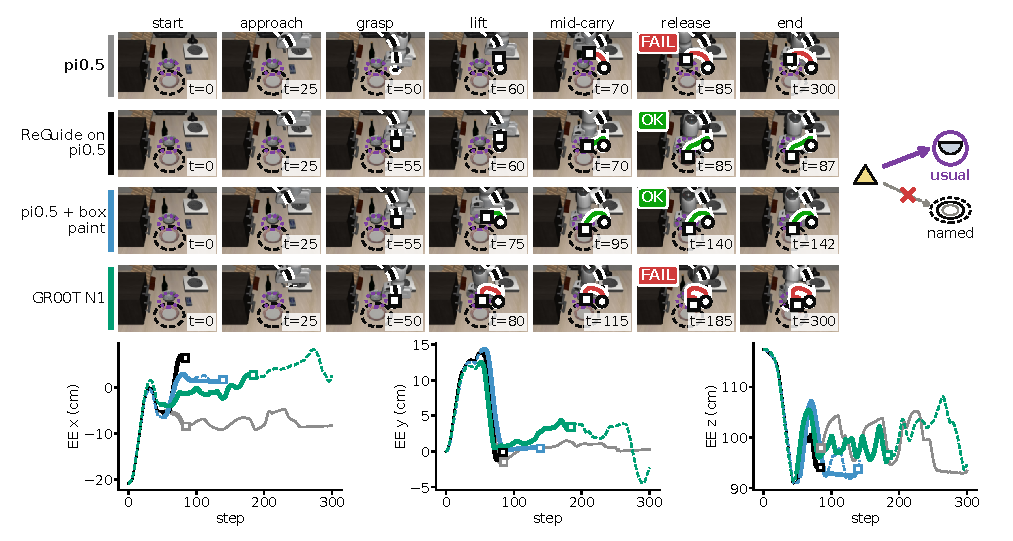
\includegraphics[width=\textwidth,]{figA2.pdf}
\caption{F1 in scene 1, three arms. Frozen \pifive{} on N1 (cream cheese on the plate): start, approach, grasp, lift, mid-carry, release, end, with the end-effector path, an outcome stamp, the cue schematic and the (x, y, z) trace against step. Rows: \pifive{} (carries to the bowl and fails), ReGuide with perceived poses (.929), and the front end tvpb (.938 against .454); GR00T N1 breaks too (E +.500). Registered: E +.450 [.28, .61]. Frames follow the frame rule of Appendix~\ref{app:A}.}
\label{fig:A2}
\end{figure}

\begin{figure}[t]
\centering
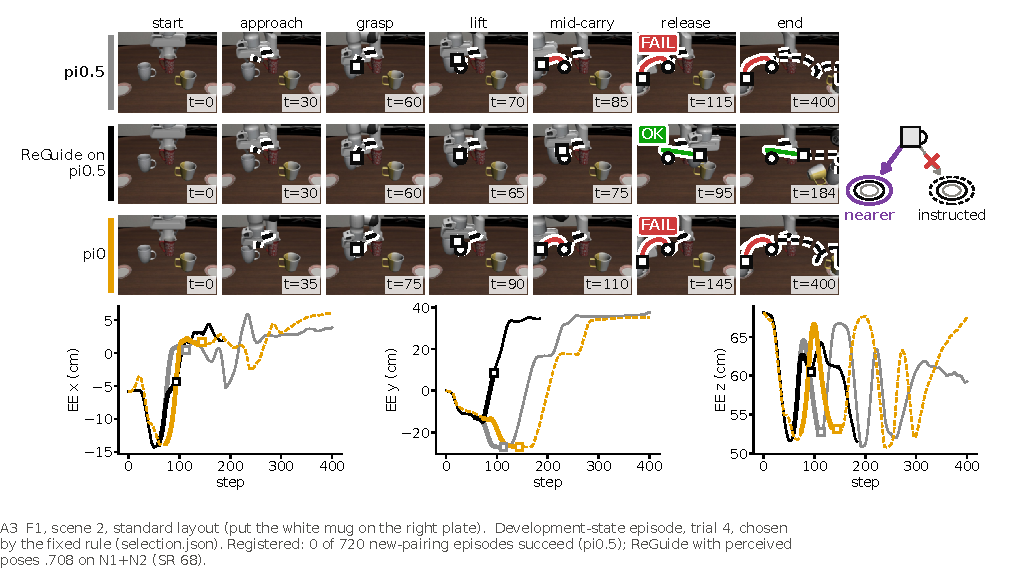
\includegraphics[width=\textwidth,]{figA3.pdf}
\caption{F1 in scene 2. Frozen \pifive{} on N1 (``put the white mug on the right plate''); 0 of 720 held-out-pairing episodes succeed in scene 2. Rows: (a) the standard layout, (b) the two mugs swapped (287 of 287 placements go to the start-side plate), (c) the plates moved (the nearer plate wins; 0 of 116 and 0 of 125 disagreeing placements go to the start-side plate). The comparator is ReGuide with perceived poses (.708 on N1 and N2; N2 1.00). \pizero{} places on the start side on .993 of 145 placements.}
\label{fig:A3}
\end{figure}

\begin{figure}[t]
\centering
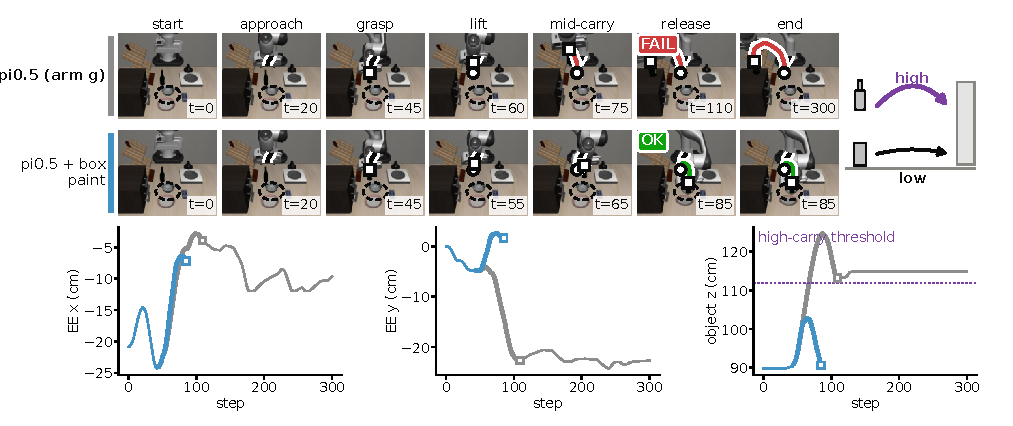
\includegraphics[width=\textwidth,]{figA4.pdf}
\caption{F1m, the held outline picks the carry. Frozen \pifive{} on N6 (bottle in the bowl; the N4 entry had no qualifying trial in the first 10) with the z profile of the carry against the high-carry threshold (lift while held above .22 m). Rows: arm g (high-carry share .225, N4+N6 success .625) and the same weights with the held bottle painted as its box, arm sb (.062 and .812). After a high carry \pifive{} succeeds .04, after a low carry .66.}
\label{fig:A4}
\end{figure}

\begin{figure}[t]
\centering
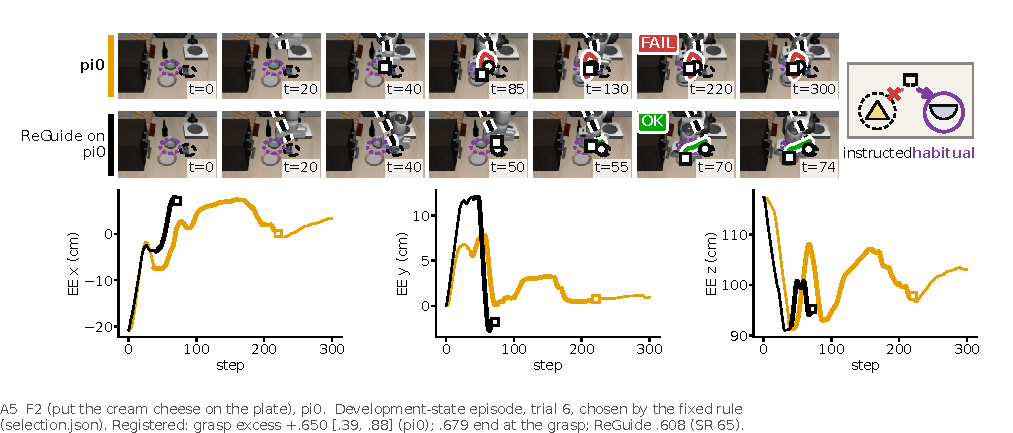
\includegraphics[width=\textwidth,]{figA5.pdf}
\caption{F2, the habitual object is grasped. \pizero{} and SmolVLA on held-out pairings (N1 cheese on the plate; N4 for SmolVLA; \pizero{} N4 had no qualifying trial in the first 10). The model grasps the scene's habitual object, outlined as the grasped object, and the episode ends at the grasp. Registered: grasp excess +.650 [.39, .88] (\pizero) and +.833 [.67, .96] (SmolVLA); .679 and .829 of held-out-pairing episodes end at the grasp; ReGuide approach transport .608 and .604; frozen \pifive{} grasps the named object at .950--.992.}
\label{fig:A5}
\end{figure}

\begin{figure}[t]
\centering
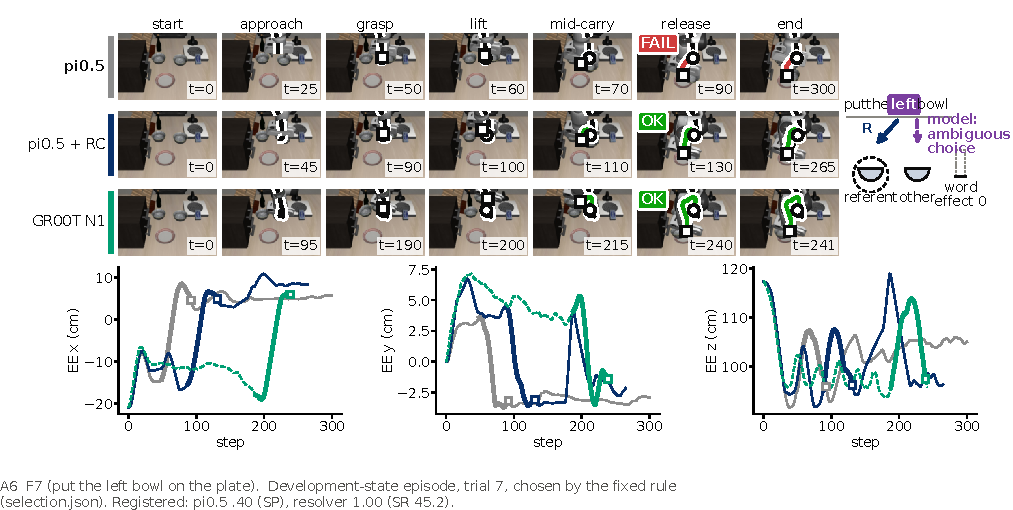
\includegraphics[width=\textwidth,]{figA6.pdf}
\caption{F7, relational and negated language is ignored. Frozen \pifive{} in scene 1 with two identical bowls, on ``put the left bowl on the plate'', ``put the right bowl on the plate'' and ``put the bowl that is not on the plate on the stove''. The model picks the bowl it picks for the ambiguous instruction on 92.5--100\% of states. Comparator: the resolver composite RC, shown with the simulator render and the painted view. Registered success: \pifive{} .40 (SP) and .20 (NG); with the resolver 1.00 and .775.}
\label{fig:A6}
\end{figure}

\begin{figure}[t]
\centering
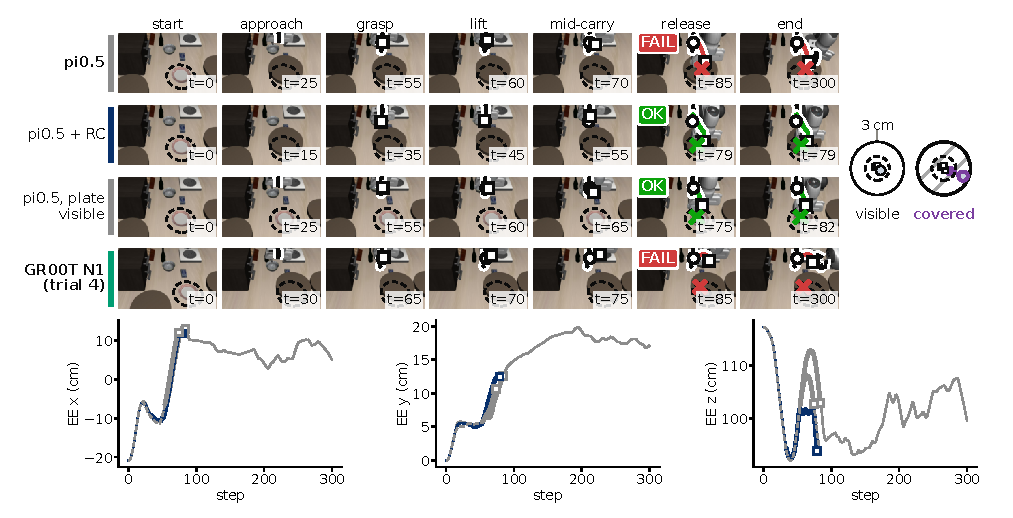
\includegraphics[width=\textwidth,]{figA7.pdf}
\caption{F6, a target seen once and then hidden. Scene 1 K1 ``put the bowl on the plate'' with the plate displaced. Columns: the first query with the plate visible, mid-carry with the cover on the plate, release. Rows: frozen \pifive{} (cost of covering, d \mi{} b, .38 [.28, .48]), GR00T (F6\_b .142 [.083, .208], cost +.60; 76\% of its failures release 3--10 cm or farther) and RC with the pose memory (.800 against .517 intact; the ghost plate is a memory overlay drawn in the simulator render only).}
\label{fig:A7}
\end{figure}

\begin{figure}[t]
\centering
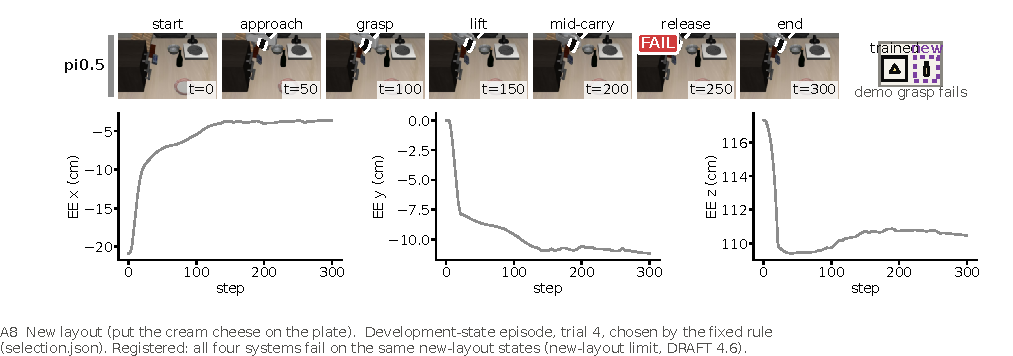
\includegraphics[width=\textwidth,]{figA8.pdf}
\caption{The held-out layout limit. Scene 1, N1 and N6 in the held-out layout, frozen \pifive{} and the scripted servo and P\_min run on the same states: all four systems fail on the same states, so the failure belongs to the task and not to the model. The demo's fixed top-down grasp holds on 0 of 10 cheese and 0 of 10 bottle states. The ghost gripper is the demo grasp pose. There is no comparator in this figure.}
\label{fig:A8}
\end{figure}

\begin{figure}[t]
\centering
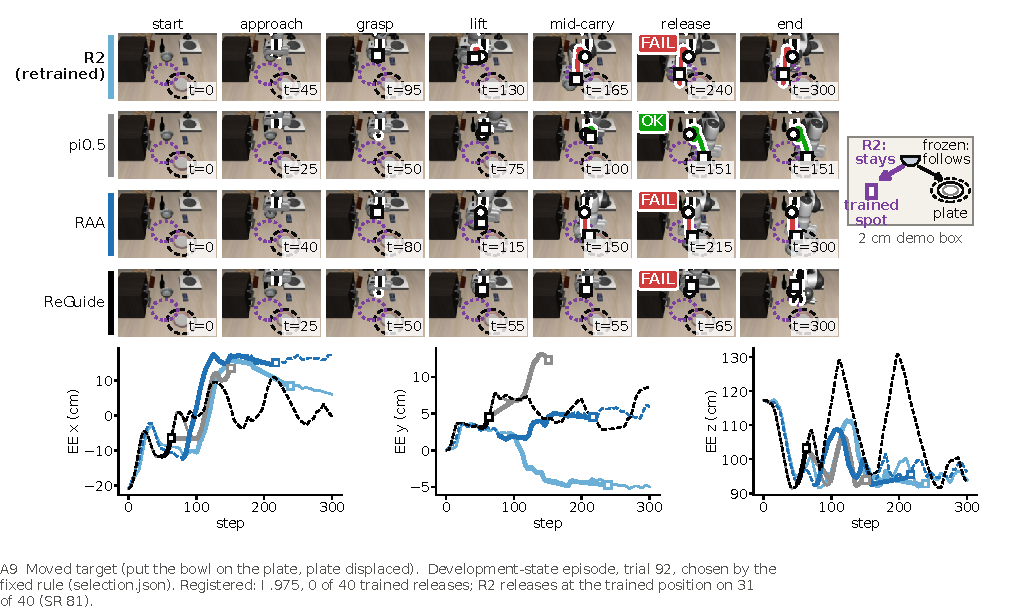
\includegraphics[width=\textwidth,]{figA9.pdf}
\caption{A moved target, frames. Scene 1 K1 with the plate .141--.296 m from the training centre (40 states). Rows: frozen \pifive{} (follows the plate; .975 success, 0 of 40 release at the trained position), the narrow retrain R2 (releases at the trained plate position on 31 of 40, median 20.2 cm off), RAA (.100) and ReGuide with perceived poses. A ghost ring marks the trained position, and a line joins each release to it. Registered numbers are in Figure~\ref{fig:A12}.}
\label{fig:A9}
\end{figure}

\begin{figure}[t]
\centering
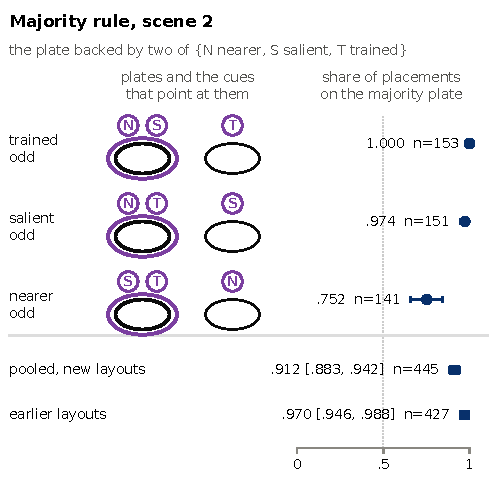
\includegraphics[width=0.6\textwidth]{figA10.pdf}
\caption{The scene-2 cue, a majority rule. Schematic of the three cues (nearer, salient, trained) and the plate chosen in each configuration. The place goes to the plate backed by two of the three: .912 [.883, .942] of 445 two-against-one placements pooled; the trained plate is outvoted on 153 of 153; the salient plate wins .974 [.947, .994] of 151 and the nearer plate .752 [.660, .843] of 141 of their respective configurations.}
\label{fig:A10}
\end{figure}

\begin{figure}[t]
\centering
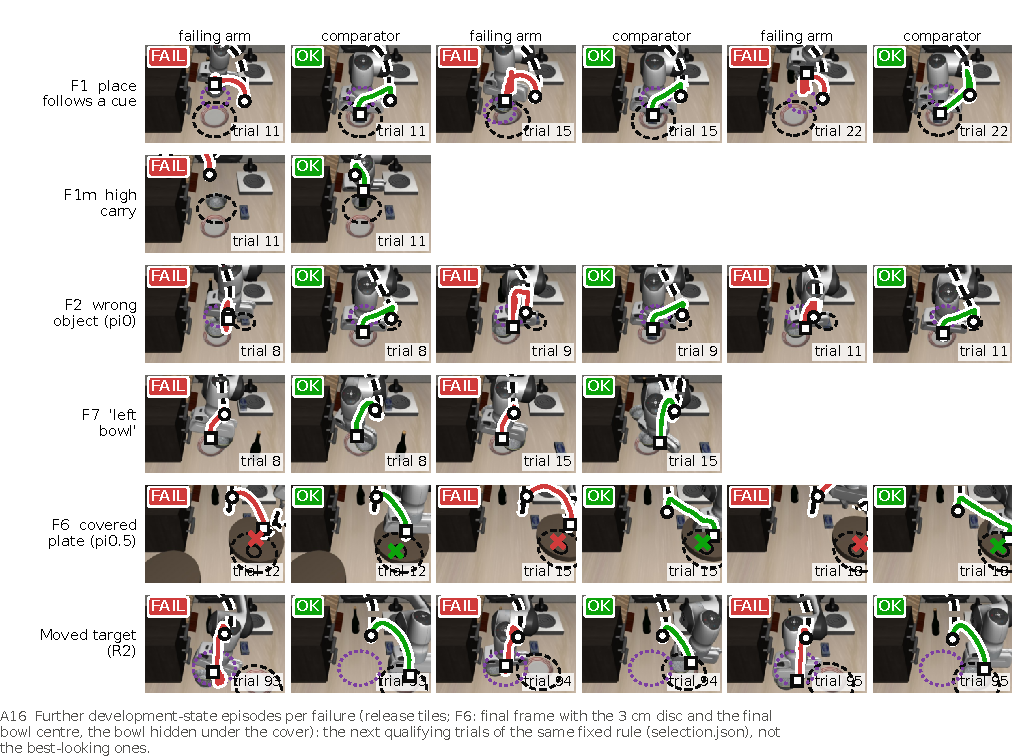
\includegraphics[width=\textwidth,]{figA16.pdf}
\caption{Frame gallery, extra episodes. Three further episodes per failure, the next three qualifying trials under the same fixed rule as Figure~\ref{fig:gallery}, shown as a thinner grid to guard against a cherry-picked look. Registered rates are those of Figure~\ref{fig:gallery}. All are development-state episodes chosen by outcome, not by appearance.}
\label{fig:A16}
\end{figure}

\clearpage
%=====================================================================
\section{The module-owned where and the removal test in detail}
\label{app:C}

\begin{table}[h]
\caption{The W1--W6 chronology (serving-time changes of the RAA-sL checkpoint, no retraining). Development states unless stated.}
\label{tab:C1}
\centering
\footnotesize
\begin{tabularx}{\textwidth}{@{}lXX@{}}
\toprule
variant & what the module owns & outcome \\
\midrule
W1 & xy of every chunk row while the role is the target (saturating servo, gain 46.875/m, clip at 2 cm) & covered plate F6 .017 to .817; trained tasks \mi.408 [\mi.720, \mi.119] (K1--K6 .528); K3 .967 to 0, K5 .683 to 0 \\
W2 & W1 plus a closed-gripper command while the bowl is more than 2 cm from the target & F6 .900; K1--K6 .542; unique-name controls .458 fail their gate \\
W3 & xy only while the held object stands at least 3 cm above the target's reference height & K3 0 to .967, K4 .283 to .983, N3 .333 to .850; K1--K6 .814; N1--N6 .922; F6 .717; K5 .067 \\
W4 & W3 plus W2's release gate & N1--N6 .928 (non-inferior to ReGuide, +.025 [\mi.053, +.111]); K1--K6 .819; F6 .867; K5 .067; controls .467 \\
W5 & release-point aim C1 (servo input minus the class's median release offset $\mu$) plus 3 cm hand-off C2 & held-out set 1: N1--N6 .892, K5 .950, covered plate .650; non-inferiority to ReGuide not shown \\
W6 & release envelope plus target latch & held-out set 2: N1--N6 .764 against .931 for W5 (\mi.167 [\mi.392, \mi.011]); cabinet-top N2 .317; latch a null (+.008 [\mi.028, +.061]) \\
\bottomrule
\end{tabularx}
\end{table}

\begin{figure}[t]
\centering
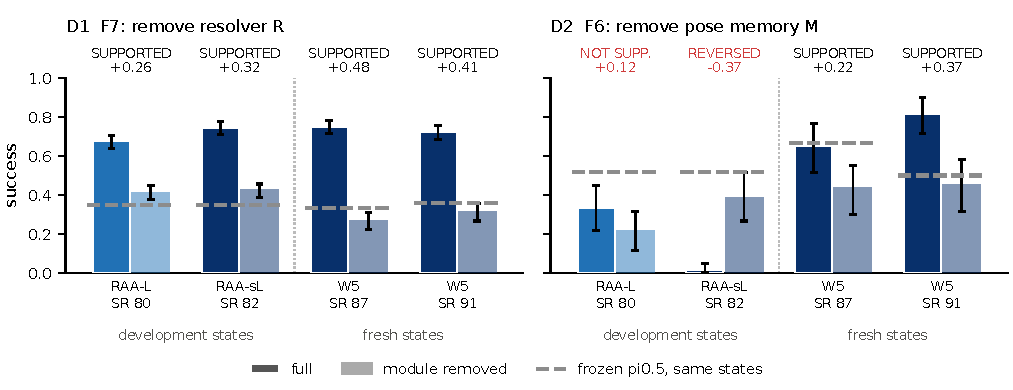
\includegraphics[width=\textwidth]{fig_removal2.pdf}
\caption{Removing one module returns one failure: success with the module (solid) and without it (hatched) on development states (RAA-L, RAA-sL) and on held-out sets 1 and 3 (RAA-sL-W5, the RAA-sL checkpoint served with the W5 where-module). Left: pooled relational (F7) cells with and without the resolver R; gain +.263 [+.213, +.313] (RAA-L), +.319 [+.269, +.375] (RAA-sL), +.483 [+.425, +.538] (W5, set 1), +.408 [+.350, +.463] (W5, set 3). Right: covered-plate cell (F6, b) with and without the pose memory M; gain +.117 [\mi.017, +.250] (RAA-L), \mi.367 [\mi.500, \mi.250] (RAA-sL, first seed; the sign reverses, and a second training seed does not reproduce it: \mi.067 [\mi.200, +.083]), +.217 [+.033, +.383] (W5, set 1), +.367 [+.217, +.517] (W5, set 3). Bars are registered 95\% intervals; the dashed line is frozen \pifive{} (.350 F7 pool, .517 F6). Held-out cells have 60 states and one seed; held-out set 2, which runs the module variant W6 (resolver +.504 [+.454, +.554], memory +.400 [+.267, +.550]), is in Table~\ref{tab:removal}.}
\label{fig:removal}
\end{figure}

\begin{table}[h]
\caption{Drop in success from removing one module (95\% intervals, 60 states per cell, one seed) on three held-out state sets: the resolver on the relational cells, the memory on the covered-plate cell. Set 2 runs the module variant W6. Every gate is testable on all three sets.}
\label{tab:removal}
\centering
\footnotesize
\begin{tabular}{@{}lll@{}}
\toprule
held-out set & remove resolver (relational cells) & remove memory (covered plate) \\
\midrule
1 & +.483 [+.425, +.538] & +.217 [+.033, +.383] \\
2 (W6) & +.504 [+.454, +.554] & +.400 [+.267, +.550] \\
3 & +.408 [+.350, +.463] & +.367 [+.217, +.517] \\
\bottomrule
\end{tabular}
\end{table}

Diagnoses behind the steps: under W1 the held object has moved 3 cm sideways 4--5 steps after the lift and touches the elevated target while more than 5 cm away (K3 20 of 20; K5 16 of 20 stall); demonstrations begin xy transport at a median 7.5 cm below the target's reference height. The rack's reference lies 12.5 cm in xy from where demonstrations release the object, against 0.9 (plate), 3.5 (stove) and 5.3 cm (cabinet). The module's held-object estimate has median error 0.95 cm and p90 2.8 cm; its open-loop 5-step chunks pass through the target in 45\% of chunks starting 1--4 cm away against 11\% for the expert; success falls from .983 to .438 as channel error grows from under 0.5 to at least 2.0 cm while RAA-sL goes from 1.000 to .867. The $\mu$ table: plate (\mi0.47, \mi0.15) cm, bowl (+0.29, \mi0.03), stove (\mi3.31, \mi0.82), cabinet (+4.23, \mi3.23), rack (\mi8.94, +8.13).

\begin{table}[h]
\caption{Cells on held-out state sets 1 / 2 / 3 (60 states per cell). W6 ran on set 2 only.}
\label{tab:C2}
\centering
\footnotesize
\begin{tabular}{@{}lllll@{}}
\toprule
cell & W5 & W6 (set 2) & RAA-sL & rgp \\
\midrule
N1--N6 & .892 / .931 / .894 & .764 & .875 / .853 / .878 & .914 / .883 / .917 \\
N4 & .717 / .783 / .533 & .667 & .783 / .767 / .817 & .867 / .717 / .800 \\
N6 & .767 / .900 / .900 & .883 & .833 / .750 / .767 & .733 / .750 / .800 \\
K1--K6 & .947 / .964 / .936 & .947 & .939 / .939 / .944 & .958 / .972 / .942 \\
K5 (rack) & .950 / .967 / .950 & .833 & .650 / .667 / .767 & .817 / .883 / .733 \\
K6 & .833 / .900 / .867 & .883 & 1.000 / .967 / 1.000 & .983 / 1.000 / .983 \\
F6\_b (covered plate) & .650 / .583 / .817 & .800 & .067 / .100 / .050 & .683 / .700 / .667 \\
\bottomrule
\end{tabular}
\end{table}

On set 1, the contrasts of W5 and its components: K5 .950 against .017 (W4) and .650 (RAA-sL, +.300 [+.200, +.417]); W5c1 alone .800, W5c2 alone .017, so C1 carries the rack. C2 recovers part of the controls (W5c2 minus W4 +.083 [+.028, +.144]; F7 pool +.058 [+.017, +.100]) at F6\_b \mi.150 [\mi.267, \mi.033]. Controls stay below RAA-sL (\mi.094 [\mi.139, \mi.050]; left unique-name .683 against .933). On the covered plate W5 beats RAA-sL (+.583 [+.467, +.717]) and ties frozen \pifive{} (.650 against .667, \mi.017 [\mi.200, +.183]); on set 3 it beats it (+.317 [+.150, +.467]); pooled +.139 [+.033, +.239]. On set 1, W5 versus RAA-sL on N1--N6 +.017 [\mi.067, +.086]; K1--K6 +.008 [\mi.103, +.142].

\textbf{Replication on set 3 (registered).} N1--N6 W5 .894 against ReGuide .917 (\mi.022 [\mi.147, +.069], NOT SHOWN); W5 against RAA-sL +.017 [\mi.125, +.128]; K1--K6 non-inferiority at \mi.05 NOT SHOWN (\mi.008 [\mi.092, +.089]); F6\_b W5 .817 against .050 (+.767 [+.667, +.867]) and .500 for frozen \pifive; K5 .950 against .767 (+.183 [+.067, +.300]).

\textbf{Why W5 loses where it loses} (replays of 480 outcomes, 20 states per cell chosen because W5 failed). W5 success falls with hand-off height: .70 (0--6 cm above the target), .54 (6--9), .27 (9--12), .14 (above 12), over 111 hand-offs. On N4 the hand-off height is 11.7 cm and the arm presses the cabinet for at least 10 steps in 65\% of W5 failures against 6\% for W4. On K6 and K1 W5 crosses the hand-off radius at 5.8--6.4 cm per chunk against 2.8 and overshoots by 2.6 cm on K6 failures. On N6, 12 of 14 failures show a held-phase channel error above 5 cm. On the unique-name control the module's estimate of the held bowl grows to a mean maximum error of 5.1 cm for W5 against 2.5 for RAA-sL. W6's release gate fires in 992 of 1,581 held cabinet calls (63\%) against 160 of 821 under W5c1 (20\%), from two job files and no gate-off arm. W6 on the hidden plate .800 against .583 for W5, controls .561 against .717 for RAA-sL. N4 is W5's weakest cell on all three sets (.717, .783, .533), post hoc.

\textbf{Pooled secondary analysis (sets 1 and 2 seen before registration).} W5 minus ReGuide on N1--N6 +.001 [\mi.053, +.049] (per set \mi.022, +.047, \mi.022; non-inferior at \mi.10; NO CLEAR DIFFERENCE); W5 minus RAA-sL +.037 [\mi.020, +.090]; K1--K6 +.008 [\mi.047, +.072]; F6\_b over RAA-sL +.611 [+.539, +.683]; K5 +.261 [+.194, +.328].

\textbf{Module removal, development history.} Gates: the R0 fit gate was not rerun on set 1 (RAA-sL's K1--K6, .939, used instead). RAA checkpoint: full .888 on trained tasks, .083 on the F6 unmoved-plate control and .108 on unique-name F7 controls (frozen \pifive{} .967 on the F6 control); D1 SUPPORTED +.213 [+.131, +.300], D2 NOT SUPPORTED +.050 [.000, +.117], primary NOT SHOWN. RAA-L (LIBERO-fine-tuned initialisation): held-out .575 against .656 (\mi.081 [\mi.181, +.022], NOT SUPPORTED); gates testable (F6 control .967, controls .558, trained .958); D1 +.263 [+.213, +.313]; D2 +.117 [\mi.017, +.250] NOT SUPPORTED (full .333, below frozen \pifive's .517; channel median error on the hidden plate 5.1 cm); D3b \mi.031 [\mi.069, +.006]. RAA-sL: gates testable (.983, .600, .9625); D1 +.319 [+.269, +.375]; D2 REVERSED \mi.367 [\mi.500, \mi.250] (full .017 [.000, .050], without M .383 [.267, .517]; the reversal did not recur on seed 2, Appendix~\ref{app:J}); primary NOT SHOWN. Diagnosis (exploratory): over 523 target-role queries the channel's median error is 1.31 cm on the covered plate and 1.12 on the unhidden; releases land 3--7 cm away, 0 of 52 succeed; the last target query has median xy offset 5.4 cm (covered) against 1.4; the expert's xy opposes the servo in the second half of the target phase (cosine \mi.92, \mi.74, \mi.64); the cover (radius 11.35 cm against the plate's 6.85) hides the plate so braking fires 3--6 cm short (44 of 59 release 3--10 cm away, 2 of 59 within 3 cm). The hide-from-expert ablation was not run. Held-out set 1: gates .900, .572, .967; D1' SUPPORTED +.483; D2' SUPPORTED +.217 (.650 to .433); D3a EQUIVALENT (identical on 60 states); D3b \mi.054 [\mi.100, \mi.012] EQUIVALENT; DK NON-INFERIOR 0 [0, 0]; primary DISSOCIATION SHOWN; removing M raises 3--10 cm releases by 14 and 16 on sets 2 and 4. Set 2 (W6): gates .917, .561, .958; D3a 0 [0, 0], D3b \mi.033 [\mi.075, +.008]. Set 3: gates .975, .561, .917; F6 b .817 to .450; D3b \mi.008 [\mi.046, +.029]; primary DISSOCIATION SHOWN. The relational ``position'' template scores 0 for every non-composite arm.

\textbf{Scene 2.} W5 and RAA-sL on scene 2, 60 states per cell, one seed. The fit check failed for the unprivileged channel, so the registered channel is the simulator's (object and target positions and in-hand offset privileged; channel error 0). Without that channel W5-S2 scores 0 of 60 on K1 and N1+N2 falls from .817 to .008. K1+K2 .700 for W5-S2, K2 weakest (.483 W5-S2, .55 RAA-sL-S2). N1+N2: W5-S2 .817 against .708 for ReGuide (+.108 [+.017, +.200], SUPPORTED by the lower bound; not like for like since W5-S2's channel and views are privileged); against RAA-sL-S2 (.792) +.025 [\mi.050, +.108] INCONCLUSIVE. K1+K2 .700 and .742 against .992 for ReGuide. D1' SUPPORTED +.433 [+.358, +.517] (K1+K2 to .325). The held-estimate share is at most .149 against a gate of .20, so D2' and the gated dissociation are UNTESTABLE.

\begin{figure}[t]
\centering
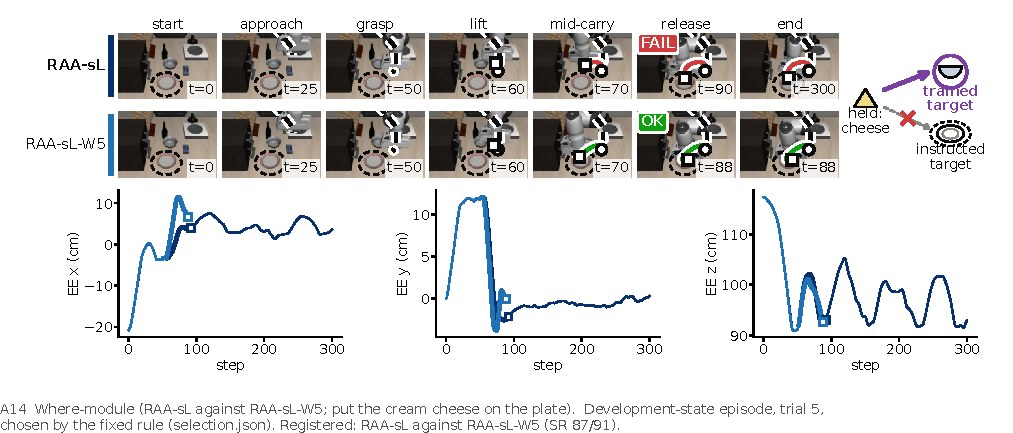
\includegraphics[width=\textwidth,]{figA14.pdf}
\caption{Where-module trace. End-effector paths with and without the servo (RAA-sL against RAA-sL-W5) and release-error histograms (N4 needed the extra 10 trials, since no trial qualified among the first 10). Registered: W5 .892 against .875 for RAA-sL on N1--N6 (set 1) and .894 against .878 (set 3); K5 .950 against .650 (set 1) and .767 (set 3) for RAA-sL; W5 is not shown non-inferior to ReGuide with perceived poses (\mi.022 [\mi.114, +.047] on set 1, \mi.022 [\mi.147, +.069] on set 3). The repair gap to ReGuide stays open.}
\label{fig:A14}
\end{figure}

%=====================================================================
\section{Activation patching on frozen \pifive}
\label{app:D}

The probe replays recorded inputs open loop and patches one write at a time from a counterfactual run (instruction names another target) into the clean run, over the 72 attention and MLP writes of the 18 VLM and 18 action-expert layers. The 124 observations come from F7 (40), held-out pairings N (48) and trained tasks K (36). The registered claim was a distributed binding: the largest write under .3 of the positive effect and a participation ratio, as a share of the 72, of at least .2. Total effect 1.658 [1.348, 1.955]. Largest write .189 [.167, .209] (action-expert layer 14 attention); participation ratio .155 [.133, .185], below .2, so the criterion is not met; the effect does not localise (largest write far under .5). The F7 set is untestable for the share statistics: a left-right swap moves the chunk by .004 [\mi.002, .011]; N and K respond (total effect 1.565 and 3.620). Of 10 band-by-set cells with a measurable intact effect none is selective and 4 are inverse: zeroing the early VLM band or either expert band raises F7's correct-target displacement, and the late expert band (layers 9--17) removes .91 of the trained tasks' displacement and leaves F7 unchanged or higher. Residual-stream patches (descriptive): patching the VLM residual at layers 0--12 transfers the full effect (1.66 to 1.53), falling from 1.21 at layer 13 to .10 at layer 14; RAA-sL .45 to .05. The expert reads the prefix through the keys and values of layer 14. Limits: one noise draw per observation, two models, one scene family, single writes sum to more than the total (coverage 2.13). On RAA-sL: largest write .180 [.141, .230], participation ratio .202 [.148, .254]; servo input plus state token .871 [.834, .914] (bar .7); servo alone .878; token \mi.007; .987 on held-out pairings, .841 on trained tasks, \mi.006 on F7; selectivity .23 [.04, .44], short of the registered margin. Band shares for \pifive: early VLM .167, late VLM .256, early expert .075, late expert .502. A targeted registered patching test of instruction-token versus cue-token keys and values at layer 14 is a possible follow-up that we have not run.

\begin{figure}[t]
\centering
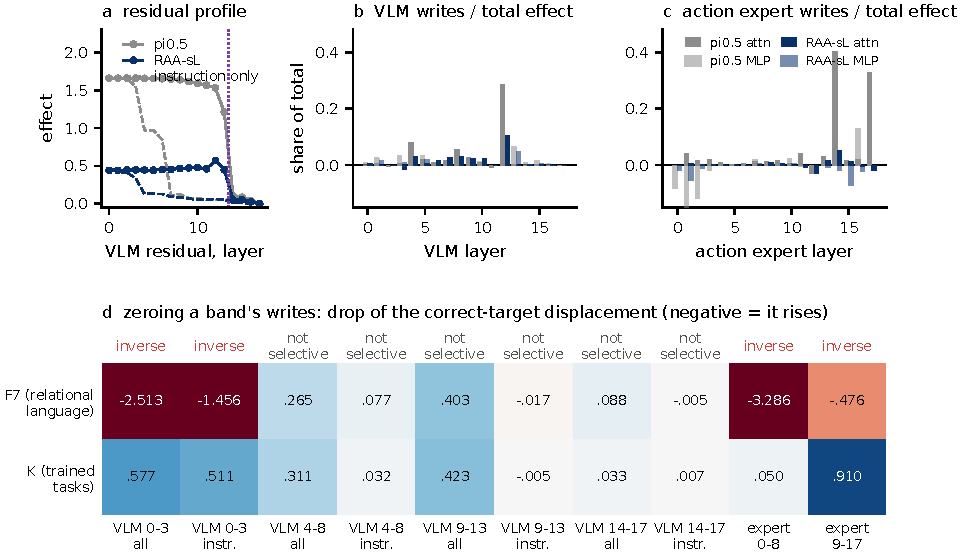
\includegraphics[width=\textwidth]{figA13.pdf}
\caption{Probe profile. (a) Layer profile of the residual-stream patch for \pifive{} and RAA-sL, whole prompt (solid) and instruction tokens only (dashed): effect 1.66 to 1.53 at layers 0--12, 1.21 at layer 13, .10 at layer 14 for \pifive; .45 to .05 for RAA-sL. (b, c) Share of the total effect carried by each of the 72 writes (attention and MLP in the VLM and in the action expert, both models; largest write .189 [.167, .209], participation ratio .155 [.133, .185] for \pifive; .180 [.141, .230] and .202 [.148, .254] for RAA-sL). (d) For \pifive, the drop in the correct-target displacement when a band's writes are zeroed, by band and set (F7 relational language, K trained tasks); 10 measurable cells, none selective, 4 inverse.}
\label{fig:A13}
\end{figure}

%=====================================================================
\section{The routes in detail}
\label{app:E}

The selection rule (fixed before any run): pass when the lower bound of the pooled share on development states is at least .70, the prefix share is below RAA-sL's (.089) and the effect is positive; fail when the upper bound is under .30. A0 was trained after we found B was built servo-free too; A+0 carries its own pre-registration record and would have had its only confirmatory test on the sealed fifth set, which stays unbuilt. Contrasts: A minus A0 +.272 [+.238, +.312]; B minus A0 +.030 [\mi.034, +.089]; A+ minus A \mi.282 [\mi.322, \mi.247]; A+ minus A0 \mi.006 [\mi.012, +.001]; A+0 minus A+ +.133 [.096, .171]; A+0 minus A0 +.127 [.092, .165]; A+0 minus A \mi.150 [\mi.196, \mi.104].

\begin{table}[h]
\caption{The learned where-share by data dose and servo on \pifive{} (96 observations per route on development states, clustered bootstrap, 95\% intervals). The pass bar is .70.}
\label{tab:share}
\centering
\footnotesize
\begin{tabular}{@{}llll@{}}
\toprule
dose & servo & route & learned where-share \\
\midrule
none & kept & RAA-sL (seed 1 / seed 2) & \mi.007 [\mi.008, \mi.006] / \mi.002 [\mi.0024, \mi.0017] \\
none & off & A0 & \mi.001 [\mi.001, .000] \\
none, target crop & off & B & .022 [\mi.046, .089] \\
small (relabel, 1--9 cm) & off & A & .274 [.239, .314] \\
large (planner, 19--38 cm) & kept & A+ & \mi.007 [\mi.013, \mi.000] \\
large (planner, 19--38 cm) & off & A+0 (post hoc) & .124 [.089, .164] \\
\bottomrule
\end{tabular}
\end{table}

\begin{table}[h]
\caption{Development behaviour of the routes (60 states per task, one seed). F6\_b arms ran on different state sets, so comparisons are indicative.}
\label{tab:E1}
\centering
\footnotesize
\begin{tabular}{@{}lccccc@{}}
\toprule
arm & N1--N6 & K1--K6 & F6\_b & F6\_a & F7 pool \\
\midrule
RAA-sL & .878 & .936 & .017 & .983 & .744 \\
A & .778 & .994 & .433 [.317, .567] & .933 & .706 \\
B & .644 & .850 & .600 [.467, .717] & .950 & .694 \\
A0 & .686 & .831 & .383 [.250, .517] & 1.000 & .700 \\
A+ & .828 & .947 & .033 & .417 & .688 \\
A+ctrl & .631 & .814 & .000 & .000 & .413 \\
A+0 & .603 & .814 & .017 & .083 & .625 \\
\bottomrule
\end{tabular}
\end{table}

A stays non-inferior to RAA-sL on K1--K6 (+.058 [\mi.006, +.167]); A+ is \mi.050 [\mi.192, +.061] below on N1--N6 with K1--K6 +.011 [\mi.028, +.067]. The relabel adds +.164 [+.006, +.403] on K1--K6 and +.194 [+.050, +.367] on the bottle pairings over A0. The F6\_b rise over RAA-sL (+.417 for A, +.367 for A0) is already in A0, so it comes from removing the servo (A minus A0 +.050 [\mi.100, +.217]); B adds +.217 [+.050, +.383] over A0 through the prefix, with no learned share. F6\_a is low (A+ .417, A+ctrl .000, A+0 .083) only for the models trained on table-spot data. A+0 against RAA-sL: N1--N6 \mi.275 [\mi.447, \mi.119] (REVERSED), K1--K6 \mi.122 [\mi.308, +.008] (NOT SHOWN), F7 \mi.119 [\mi.188, \mi.044] (REVERSED); against A+ N1--N6 \mi.225 [\mi.386, \mi.078]. The prefix half of the pass rule fails every servo-free route by construction: RAA-sL's prefix share is .089 because its effect runs through the servo outside the network, and a servo-free route has no outside path (A0 reads 1.002, A .751, lower than A0 by .250 [.218, .285], and B 1.001). A+ctrl's Phase B used a new serving copy with a zero state and learned masks, unlike Phase A. The relabel cannot reach the 20--40 cm scale of a real mis-pairing, because shifts must stay in the support of the demonstrations. Alternative explanation for A+'s null: the new prompt phrase on the table-spot frames; A+0 keeps the phrase and rises to .124, so the servo accounts for the zero. The oracle frames (Appendix~\ref{app:K}) show that A+0 and A follow the token where only the token decides ($\varphi$ .771 and .662), and \pizero{} with a trained state pathway reads the token with no dose, so these null shares apply to a newly added pathway.

\begin{figure}[t]
\centering
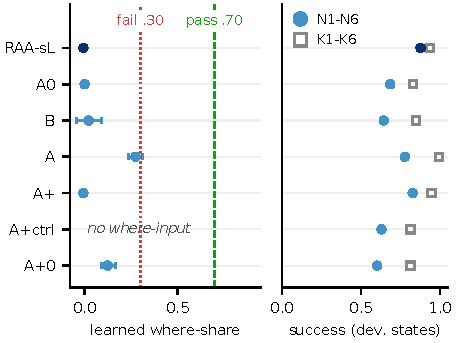
\includegraphics[width=0.7\textwidth]{figA15.pdf}
\caption{The routes as dots. The \pifive{} routes of Section~\ref{sec:grid} as a dot plot: learned where-share and N1--N6 success. Where-share: RAA-sL \mi.007, A0 \mi.001, B .022, A .274 [.239, .314], A+ \mi.007, A+0 .124 [.089, .164]. N1--N6 success: RAA-sL .878, A .778, B .644, A0 .686, A+ .828, A+ctrl .631, A+0 .603 (K1--K6 .814). A+0 is a post hoc route. Development states; one seed.}
\label{fig:A15}
\end{figure}

%=====================================================================
\section{The moved plate in detail}
\label{app:F}

Plate cells span 4.0--6.9 cm (near) and 14.1--28.9 cm (far); bowl cells 4.2--6.9 and 14.6--29.7 cm for K1 and 4.1--6.9 and 14.5--29.6 cm for K2. The registered prediction that frozen \pifive{} shows a trained-release share above 0 reads NOT SUPPORTED (M1, predicted at 85\%); M1 is weak by construction, since the in-range share is 0 by the 3 cm rule. R2 in range reaches .675 [.525, .825], below the .70 floor. RAA minus frozen \pifive{} \mi.875 [\mi.975, \mi.750] reads REVERSED against the prediction (M2). With the bowl .14--.30 m away, frozen \pifive{} succeeds on .375 [.225, .525] of K1 and .400 [.250, .550] of K2, against .850 and .925 for ReGuide with perceived poses (+.475 [+.275, +.650] and +.525 [+.375, +.675]). The record does not say where the arm goes when the grasp fails; the reach attribution is confounded by the approach path.

\begin{figure}[t]
\centering
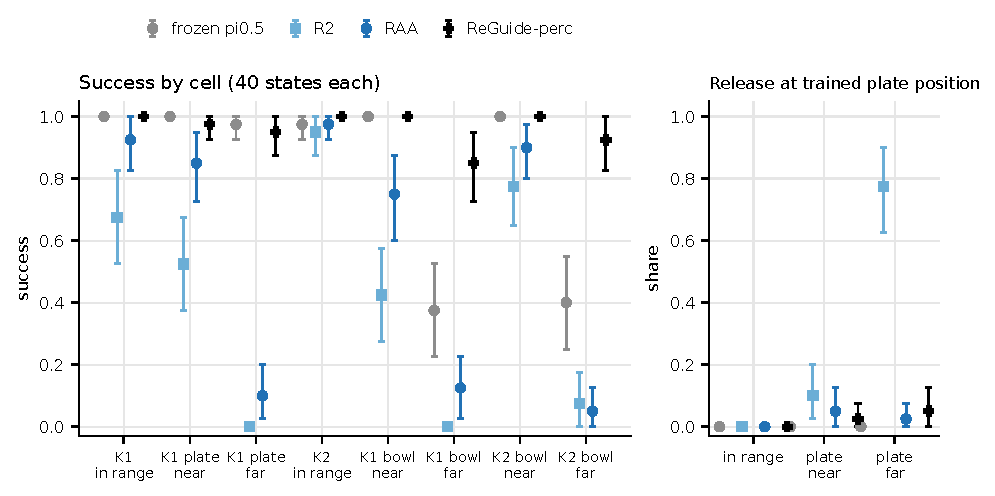
\includegraphics[width=\textwidth]{fig_moved.pdf}
\caption{A moved target: frozen \pifive{} follows the plate, a narrow retrain releases at the trained position. Left: success of frozen \pifive, the narrow retrain R2, RAA and ReGuide with perceived poses, on eight cells of 40 states each. K1 puts the bowl on the plate and K2 puts it on the stove. ``Plate'' cells move the plate, and ``bowl'' cells move the bowl, by a near or far distance. Right: the share of episodes whose release lies more than 3 cm closer to the trained plate position than to the actual plate, on K1 with the plate moved; the share is 0 by construction in range. Bars are 95\% bootstrap intervals from the registered read. Figure~\ref{fig:A9} shows the frames.}
\label{fig:A12}
\end{figure}

%=====================================================================
\section{A steerability predictor (failed its registered test)}
\label{app:G}

The probe sends, at every query of a closed-loop rollout of a trained task, a side query on the same observation with one word swapped (object word in the grasp phase, target word in the place phase). A query scores 1 when the first five steps of the chunk point nearer the swapped-in entity; steerability $g_s(o)$ and $p_s(t)$ average that, and the prediction is the product $g_s(o) p_s(t)$ (the product form of \citealt{okawa2310}). We use 16 policies in scene 1 and 3 in scene 2, with 10 states per trained task. The registered headline on the 24 wrapper-free cells gave AUC .550 [.000, 1.000], Spearman .227 [\mi.440, .812] (NOT SUPPORTED); across 15 policies the Spearman with N1--N6 success is .193 [\mi.424, .736] (NOT SUPPORTED); trained-task success alone gives AUC .800 on the four wrapper-free policies; the scene-2 test failed its bar.

\begin{table}[h]
\caption{Steerability scores against held-out success.}
\label{tab:G1}
\centering
\footnotesize
\begin{tabular}{@{}llll@{}}
\toprule
score & cells & AUC & stage \\
\midrule
steerability, wrapper-free policies & 24 & .550 [.000, 1.000] & registered headline \\
steerability, scene 1 & 90 & .742 [.526, .907] & registered, missed .75 by .008 \\
trained-task success alone & 90 & .645 [.419, .846] & baseline \\
nonsense-word sensitivity & 90 & .462 [.240, .684] & baseline \\
k $\times$ a (success times floor-corrected steering) & 90 & .787 & post hoc \\
k $\times$ a, Rrel and RAA & 12 & .944 [.667, 1.000] & pre-registered, new policies \\
k $\times$ a, all policies & 102 & .805 [.603, .940] & pre-registered, new policies \\
trained-task success alone, Rrel and RAA & 12 & .500 & baseline \\
\bottomrule
\end{tabular}
\end{table}

Two problems explain the failure: the angle rule has a floor (.22--.28 of scene-1 queries point nearer the swapped-in entity under the true prompt), and the entity decides most of the score (swaps to the bottle .13--.47; to the bowl target .00--.46). Subtracting the floor raises the 90-cell AUC to .770; k $\times$ a gives .787 and Spearman .579; entity normalisation lowers it to about .60--.65. The confirmation covers two policies from one base, six pairings and one scene; its lower bound of .667 sits below the .75 bar and both policies sit at .94 trained success. Pooled Spearman .575 [.254, .756]; the score ranks RAA above Rrel (.364 against .301) as their success does (.656 against .278); Rrel on N1 scores .393 and succeeds on 0. Within GR00T variants Spearman is .922 over 18 cells. ReGuide, Hp and RC lie outside the probe. Related predictors: \citet{okawa2310} (product form), STAGE \citep{stage2609} and LIBERO-PRO (sensitivity probes), and world-model evaluators \citep{veo2512}.

%=====================================================================
\section{Ladder details}
\label{app:H}

\begin{table}[h]
\caption{Matched-data results on 60 states per task in scene 1. RAA-s adds a fixed servo residual on the translation dimensions of each chunk to RAA. RAA-sL starts RAA-s from the LIBERO-fine-tuned \pifive, and the other retrains start from the base weights. ReGuide (rgp) is the external reference.}
\label{tab:ladder}
\centering
\footnotesize
\begin{tabular}{@{}lcccc@{}}
\toprule
variant & N1--N6 & right grasp & placed given right grasp & K1--K6 \\
\midrule
R0 & .042 & .417 & .100 & .853 \\
R2 & .389 & .972 & .400 & .753 \\
Rrel & .278 & .861 & .323 & .911 \\
RAA & .656 & 1.000 & .656 & .839 \\
RAA-s & .717 & .967 & .741 & .844 \\
RAA-sL (seed 1 / seed 2) & .878 / .822 & .997 / 1.000 & .880 (seed 1) & .936 / .856 \\
rgp (ReGuide) & .897 & .989 & .907 & .950 \\
\bottomrule
\end{tabular}
\end{table}

RAA beats R2 on placed given right grasp by +.256 [+.077, +.461]; the cheese pairings gain +.322 [+.005, +.717] and the bottle pairings +.211 [+.078, +.367]. V3: RAA trails ReGuide by \mi.242 [\mi.464, \mi.033], missing the \mi.10 margin. Contact-induced training roles: all 300 routed demonstrations had a hold event; the channel stays within 1 cm of the simulator for 69\% of object-role and 89\% of target-role queries (medians 0.30 and 0.06 cm). On N4 and N6, Rrel grasps the right object on .733 and .567 of episodes. In the exploratory diagnostic (160 episodes), ReGuide's median release error is 0.9--1.7 cm and RAA's failed releases miss by 3.7--7.9 cm; on the bottle pairings the error tracks the held object's offset (r = .57 on N4). RAA-o: r = .14 (N4), .03 (N6), error N4 6.5 against 7.0 cm; trails ReGuide \mi.303 [\mi.481, \mi.111]; NOT SUPPORTED. RAA-c: median error of the fed target .94 cm; trails ReGuide \mi.394 [\mi.608, \mi.158]; known-task .814 against .881 (\mi.067 [\mi.233, +.061]); failed releases N4 11.8 against 6.5 cm; NOT SUPPORTED. RAA-s (re-serve with the servo after a serving bug that omitted it): .717 against .656, .594 and .503, trained .844; PARTIAL (+.122 [\mi.019, +.264]); placed given right grasp +.140 [+.008, +.280]; bottle pairings +.261 [+.133, +.400], cheese \mi.017 [\mi.133, +.067]; over RAA-c +.214 [+.075, +.381]; over RAA +.061 [\mi.117, +.253]; failed bottle releases 6.5 (N4) and 3.8 cm (N6) against 11.8 and 11.0 for RAA-c; ReGuide leads by \mi.181 [\mi.300, \mi.055]; trained-task non-inferiority NOT SHOWN (\mi.036 [\mi.178, +.075]). RAA-sL: .878, trained .936, right grasp .997; against RAA-s +.161 [\mi.017, +.311] NOT SUPPORTED; against RAA-L (.575) +.303 [+.042, +.567] SUPPORTED; bottle pairings .883 against .589 (+.294 [+.183, +.400]); cheese +.028 [\mi.167, +.267]; trained +.092 [+.011, +.200]; against ReGuide \mi.019 [\mi.106, +.061], non-inferiority at \mi.10 NOT SHOWN (lower bound .006 under the margin); N4 18 of 20 against 13.

\begin{figure}[t]
\centering
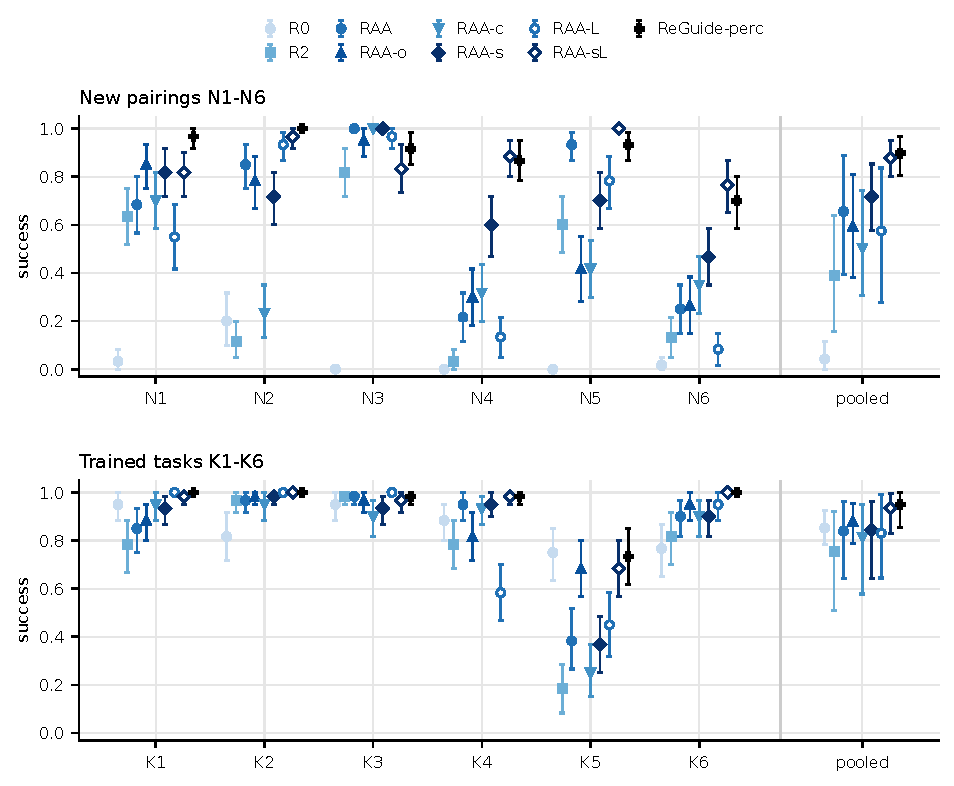
\includegraphics[width=\textwidth]{fig_arms.pdf}
\caption{Success of every trained variant, per task. Top: the six held-out pairings N1--N6 and their pool. Bottom: the six trained tasks K1--K6 and their pool. Each point is success over 60 states of one task (one seed per variant). Bars are 95\% percentile intervals from a cluster bootstrap over tasks and states (B = 2000): the pooled bar resamples the six tasks, then the 60 states within each drawn task, so it carries task-level spread; the per-task bars resample the 60 states of that task. R0 and R2 are plain retrains, RAA adds the role channel, RAA-o measures the target from the held object, RAA-c feeds the offset as a state token, RAA-s adds a servo term, and RAA-L and RAA-sL (open markers) start from the LIBERO-fine-tuned \pifive. ReGuide with perceived poses (black) is the external reference.}
\label{fig:A11}
\end{figure}

%=====================================================================
\section{Prior art and limits, extended}
\label{app:I}

Each component exists: FOCI predicts motion in an object-relative frame; OA-WAM (relative-pose bias between object slots and robot slot, the closest precedent for our channel) and POT-VLA feed object tokens or role-indexed records to an action expert; w$^{2}$VLA \citep{w2vla2606} injects a language-conditioned location through FiLM; AC-VLA and LiLo-VLA restrict the input by gripper phase. We read FOCI, OA-WAM and POT-VLA in full text through a summarising fetch and the others by abstract. Other limits not in the main text: the hand-over idea has prior art in ReGuide, Harness VLA and LiLo-VLA; MEM and \pizero.7 add memory by training; no hand-over variant of ours clears the .50 bar and holds trained tasks; we ran no placement checks on the F7 and F6 states of held-out sets 1--3; the causes of W5's failures come from replays of selected states; no effect was found from chunk length or release timing; we did not reproduce the partner-count law of \citet{wang2607} on two frozen VLAs; the new-layout limit carries no VLA claim; the recipe's fixed constants are one gain (fitted to the demonstrations by least squares), one clearance, one hand-off radius and one release table (read from the demonstrations). Memory and occlusion benchmarks exist for the covered-target failure: RoboMME \citep{robomme2603} covers temporal, spatial, object and procedural memory, and LIBERO-Mem \citep{liberomem2511} covers object-level partial observability. We ran neither.

%=====================================================================
\section{Second training seed of RAA-sL}
\label{app:J}

We trained RAA-sL again with seed 43 (seed 1 used the config default 42). The seed also changes the random initialisation of the state-projection layer and the data order. Everything else is as in the main RAA-sL run: data, norm stats, servo constants, 6,001 steps, the same states (development states; no held-out state set is involved) and the same readers. We wrote the predictions and the replication rule before any seed-43 training job. The rule: N1--N6 and K1--K6 REPLICATE if the point gap is at most .05 and are CONSISTENT if the gap is larger and the two 95\% intervals overlap; D1 REPLICATES if it keeps its sign and its SUPPORTED verdict; D2 is reported with no claim; the in.tok where-share REPLICATES if its interval upper bound is under .30 and $|$point$|$ $<$ .05, and the servo and channel shares REPLICATE if each lies within .10 of seed 1.

\begin{table}[h]
\caption{Seed 1 against seed 2 (paired bootstrap on the same states, B = 2000).}
\label{tab:J1}
\centering
\footnotesize
\begin{tabularx}{\textwidth}{@{}lXXlX@{}}
\toprule
quantity & seed 1 & seed 2 & gap & verdict \\
\midrule
N1--N6 success & .878 & .822 & \mi.056 [\mi.181, +.056] & CONSISTENT \\
K1--K6 success & .936 & .856 & \mi.081 [\mi.261, +.022] & CONSISTENT \\
D1, full minus noR, F7 pool & +.319 [+.269, +.375] SUPPORTED & +.444 [+.394, +.494] SUPPORTED & & REPLICATES \\
D2, full minus noM, F6\_b & \mi.367 [\mi.500, \mi.250] REVERSED & \mi.067 [\mi.200, +.083] NOT SUPPORTED & & reported only, no claim \\
probe in.tok where-share & \mi.007 [\mi.008, \mi.006] & \mi.002 [\mi.0024, \mi.0017] & & REPLICATES \\
probe in.servo / in.chan share & .920 / .913 & .911 [.878, .946] / .909 [.876, .944] & \mi.009 / \mi.004 & REPLICATE \\
\bottomrule
\end{tabularx}
\end{table}

K gap: K5 drives it (.683 on seed 1, .200 on seed 2); K1--K4 and K6 lie within .035 of seed 1. Bottle pairings N4--N6 fall from .883 to .772 and cheese pairings N1--N3 stay at .872. P1 (against RAA-s) stays NOT SUPPORTED (+.106 [\mi.044, +.258]), P2 (against RAA-L) stays SUPPORTED (+.247 [+.064, +.445]), and P3a (against ReGuide) stays NOT SHOWN (\mi.075 [\mi.206, +.039]). PK, the K non-inferiority over RAA-s, does not recur (+.011 [\mi.086, +.078], NOT SHOWN, against +.092 [+.011, +.200] on seed 1). Full F6\_b rises from .017 to .133, still far under the unhidden F6\_a (.95) and under frozen \pifive{} (.517), so the hidden-plate failure recurs and the seed-1 collapse to 1 of 60 was partly seed-specific. D3a, D3b and DK keep their labels, and the gates stay TESTABLE (.950, .692, .975) with the gated primary NOT SHOWN. The held-target channel has median error .85 cm at test with only role ids 1 and 2 on the state lines.

\textbf{Deviation.} The registered CONSISTENT rule compares each seed's own interval. The read produces only the paired seed-2 minus seed-1 interval, so we established CONSISTENT by that interval containing 0, which implies that the two per-arm intervals overlap. We did not compute the per-arm intervals. The read script's self-test was not rerun (the machinery is unchanged). \textbf{Limits.} One extra seed, one trial per state, 60 states per Phase A task, and both seeds share all state sets, so the replication adds no confirmatory claim beyond that of the main RAA-sL run.

%=====================================================================
\section{Oracle arm and \pizero{} replication}
\label{app:K}

This appendix reports Exp 1 (an oracle arm, Section~\ref{sec:grid}) and Exp 2 (a \pizero{} replication, Section~\ref{sec:pi0}). We executed both on 2026-11-22 and 2026-11-23, each with a pre-registration row and written predictions. Each arm has one seed and all reads use development states, as every RAA-F route does.

\textbf{Design.} The \pizero{} arms use openpi's \pizero{} with its native, trained state pathway. The token (the same offset as RAA-c) enters state dimensions 0 to 3 of the trained state projection, with quantile normalisation and no delta actions (pi0\_libero as shipped predicts action minus state), so the arms deviate from \pizero{} as shipped. pi0-sL keeps the servo and pi0-A0 removes it with no added data. The checks confirm that the \pizero{} port equals openpi's Pi0 exactly, that the servo identities hold, that the parameter tree equals pi0\_libero's (50 tensors) and that the state projection is bit-equal to the shipped one.

\subsection{Follow share on oracle frames}
\label{app:K1}

131 observations, 23 layouts; clustered bootstrap, B = 2000.

\begin{table}[h]
\caption{Follow share $\varphi$ on the oracle frames.}
\label{tab:K1}
\centering
\footnotesize
\begin{tabular}{@{}llcccc@{}}
\toprule
model & $\varphi$ (95\% CI) & label & $c_{\mathrm{clean}}$ & $\varphi_{\mathrm{zero}}$ & $\sigma_{\mathrm{demo}}$ \\
\midrule
A+0 (servo off, planner dose) & .771 [.605, .887] & PARTIAL & .676 & .166 & 1.61 \\
A (small relabel, servo off) & .662 [.542, .783] & PARTIAL & .447 & .043 & 1.33 \\
A0 (no dose, servo off) & \mi.001 [\mi.002, .000] & NOT LEARNED & \mi.329 & .001 & \mi.002 \\
A+ $\varphi_{\mathrm{net}}$ (servo kept) & \mi.068 [\mi.210, .042] & NOT LEARNED & .821 & \mi.024 & \mi.168 \\
RAA-sL $\varphi_{\mathrm{net}}$ (servo kept) & \mi.006 [\mi.008, \mi.005] & NOT LEARNED & .892 & .001 & \mi.014 \\
\bottomrule
\end{tabular}
\end{table}

$\varphi_{\mathrm{total}}$ (token and servo from the counterfactual): A+ .830 [.737, .911], RAA-sL .957 [.906, 1.006], so the servo carries the where. Cluster-paired contrasts: $\varphi$(A+0) minus $\varphi$(A0) +.772 [+.606, +.887]; $c_{\mathrm{clean}}$(A+0) minus $c_{\mathrm{clean}}$(A0) +1.006 [+.819, +1.189]; $\varphi_{\mathrm{net}}$(A+) minus $\varphi$(A+0) \mi.839 [\mi1.029, \mi.665] (the servo effect on oracle frames); $\varphi$(A+0) minus $\varphi$(A) +.109 [\mi.018, +.219]. The registered gate (train ORC unless A+0 is LEARNED) fired, because the lower bound .605 of A+0 is under .70. The test set has 131 observations on 23 layouts; the registered cap of 250 attempts per object stopped generation at 16 complete pairs (bowl) and 8 (cream cheese) instead of 20 and 20, which still passes the floor of 120 observations. The replay check restores the end effector to 0.000 mm for 48 of 48 stored demonstrations.

Labels for the registered predictions: o1 (A0 $\varphi$ CI upper $<$ .30) TRUE; o2 (RAA-sL $\varphi_{\mathrm{net}}$ CI upper $<$ .30) TRUE; o3 (A+ $\varphi_{\mathrm{net}}$ CI upper $<$ .30) TRUE (.042); o4 (A+0 $\varphi$ point .50, range .15 to .85) in range with point .771, A+0 LEARNED (30\%) FALSE, A+0 NOT LEARNED (25\%) FALSE (PARTIAL); o5 (A+0 $c_{\mathrm{clean}}$ above A0 $c_{\mathrm{clean}}$, CI lower $>$ 0) TRUE.

\subsection{ORC: A+0's data plus 39 paired-spot demonstrations}
\label{app:K2}

ORC trains 6,001 steps (step-0 loss .0781) on A+0's data (400 base and 100 planner demonstrations) plus 39 paired-spot demonstrations: 7,659 held frames against 5,306 for A+0 (+44\%).

\begin{table}[h]
\caption{ORC against A+0 on the oracle frames.}
\label{tab:K2}
\centering
\footnotesize
\begin{tabular}{@{}llllll@{}}
\toprule
model & $\varphi$ (95\% CI) & label & $c_{\mathrm{clean}}$ & $\varphi_{\mathrm{zero}}$ & N + K in.tok share \\
\midrule
ORC & .777 [.628, .873] & PARTIAL & .727 & .033 & .195 [.124, .278] (N .338, K .077; in.prefix .565) \\
A+0 & .771 [.605, .887] & & .676 & .166 & .124 [.089, .164] \\
\bottomrule
\end{tabular}
\end{table}

K / N capture success for ORC: .825 / .4375. $\varphi$(ORC) minus $\varphi$(A+0) +.005 [\mi.058, +.066]; $c_{\mathrm{clean}}$ +.051 [\mi.022, +.128]; $\varphi$(ORC) minus $\varphi$(A0) +.777 [+.629, +.873]. Adding 39 paired-spot demonstrations did not move $\varphi$. We did not run ORC development rollouts, which the plan registered only if the N + K share had a lower bound of at least .70. Labels: o6 (ORC $\varphi$ point .75) in range at .777, ORC LEARNED (55\%) FALSE (CI lower .628), ORC NOT LEARNED (10\%) FALSE; o7 ($\varphi$(ORC) minus $\varphi$(A+0) CI lower $>$ 0, 65\%) FALSE; o8 (N + K share point .20) .195, CI upper $<$ .30 (55\%) TRUE, CI lower $\geq$ .70 (7\%) FALSE; o9 (within-model dissociation: the oracle model LEARNED and the N + K CI upper $<$ .30; 45\%) FALSE, because both oracle models are PARTIAL (the N + K half holds for both).

\subsection{\pizero{} fit gate and token read}
\label{app:K3}

Pooled N + K, rows full.

\begin{table}[h]
\caption{Fit gate. K success on tasks 0, 2, 6, 10; N success on tasks 16, 22, 24, 26.}
\label{tab:K3a}
\centering
\footnotesize
\begin{tabular}{@{}lllllll@{}}
\toprule
arm & K success & K pool & N success & N pool & T & gate \\
\midrule
pi0-sL (servo kept) & .95 1.0 .95 .90 & .950 & .90 .55 .95 .35 & .6875 & 4.272 [3.939, 4.610] & PASS \\
pi0-A0 (servo off) & 1.0 1.0 .85 1.0 & .9625 & .80 .00 .65 .15 & .400 & 3.044 [2.668, 3.444] & PASS \\
reference RAA-sL (\pifive) & 1.0 .95 .95 1.0 & .975 & .65 .85 1.0 .70 & .800 & & \\
reference A0 (\pifive) & 1.0 .95 .75 1.0 & .925 & .60 .40 .90 .20 & .525 & & \\
\bottomrule
\end{tabular}
\end{table}

The fit gate (K pool of at least .70 and a T interval with a positive lower bound) applied before any token read, and both arms pass.

\begin{table}[h]
\caption{Token read on \pizero.}
\label{tab:K3b}
\centering
\footnotesize
\begin{tabular}{@{}lll@{}}
\toprule
quantity & pi0-sL (servo kept) & pi0-A0 (servo off) \\
\midrule
pooled in.tok share & \mi.150 [\mi.174, \mi.127] & .542 [.478, .609] \\
N / K in.tok & \mi.147 / \mi.153 & .755 / .371 \\
in.prefix pooled & .190 & .387 \\
in.servo & .960 [.928, .994] & \\
abl.tok drop (K) & \mi.457 & +.271 \\
\bottomrule
\end{tabular}
\end{table}

Cross-backbone contrasts on in.tok: pzA0 minus pzsL +.683 [+.608, +.767]; pzA0 minus A0 (\pifive) +.531 [+.463, +.607]; pzsL minus RAA-sL \mi.143 [\mi.168, \mi.119]. The relative Frobenius change of the live state-projection columns 0 to 3 from pi0\_libero's initialisation is .0158 for pzsL and .0173 for pzA0 (pad columns exactly 0). The live columns of pi0\_libero's state projection were trained on end-effector position and the x axis-angle component, so the negative share of pzsL (\mi.150) is leftover dependence with the sign opposite to the counterfactual target, present only where the servo already supplies the correction.

Decision rules. R1 (the \pifive{} shortcut replicates on \pizero: S\_off CI upper $<$ .30): FALSE (.609). R2 (the no-dose read: S\_off CI lower $\geq$ .30): TRUE (.478); the strong form ($\geq$ .70) FALSE. R3 (the servo suppresses the token): TRUE (S\_off minus S\_kept +.68 [+.61, +.77]). R4 (the servo fails to suppress): FALSE. Labels: z1 (both fit gates pass) TRUE; z2 (S\_kept point .00, range \mi.05 to .20) point \mi.150 outside the range, CI upper $<$ .30 TRUE; z3 (S\_off point .08, range \mi.05 to .45) .542 outside, CI upper $<$ .30 FALSE, CI lower $\geq$ .30 TRUE, CI lower $\geq$ .70 FALSE; z4 (R1) FALSE; z5 (R3) TRUE; z6 (R4) FALSE; z7 (in.servo $\geq$ .70) TRUE (.960); z8 (sL K within .10 of RAA-sL's, and A0 N below sL N) TRUE (.950 against .975; .40 against .6875); z9 (A0 relative state-projection change larger than sL) TRUE (descriptive, tiny difference).

\subsection{\pizero{} development rollouts}
\label{app:K4}

Phase A K1--K6 and N1--N6 with 60 states each (trials 4 to 23 and 24 to 63), and Phase B (F7 pool, F6\_b, F6\_a), on the pipeline of the RAA-F development read. Paired clustered bootstrap, B = 2000.

\begin{table}[h]
\caption{Development rollouts of the \pizero{} arms.}
\label{tab:K4}
\centering
\footnotesize
\begin{tabular}{@{}llllllll@{}}
\toprule
arm & dev K & dev N & cheese & bottle & F7 pool & F6\_b & F6\_a \\
\midrule
pi0-sL & .811 & .761 & .939 & .583 & .638 & .000 & .733 \\
pi0-A0 & .906 & .506 & .783 & .228 & .575 & .200 & .967 \\
RAA-sL (\pifive) & .936 & .878 & .872 & .883 & .744 & .017 & .983 \\
A0 (\pifive) & .831 & .686 & .856 & .517 & .700 & .383 & 1.000 \\
\bottomrule
\end{tabular}
\end{table}

Registered contrasts on N. d1: pi0-A0 minus pi0-sL \mi.256 [\mi.386, \mi.128] (CI upper $<$ 0); K difference +.094 [+.003, +.208]; d4 (K non-inferiority at \mi.05) holds. d2: pi0-A0 minus A0 (\pifive) \mi.181 [\mi.344, \mi.008]. d3: pi0-sL minus RAA-sL \mi.117 [\mi.306, +.067] (CI straddles 0); on K \mi.125 [\mi.258, \mi.017]; pi0-A0 minus RAA-sL on N \mi.372 [\mi.633, \mi.081]. Phase B: F7 pool pi0-A0 minus pi0-sL \mi.063 [\mi.137, +.019]; F6\_b +.200 [+.100, +.300]; F6\_a +.233 [+.117, +.350]; pi0-A0 minus A0 on F7 \mi.125 [\mi.194, \mi.056] and on F6\_b \mi.183 [\mi.317, \mi.033]. Per task N (pi0-sL / pi0-A0): N1 .88/.77, N2 .93/.63, N3 1.0/.95, N4 .53/.08, N5 .87/.53, N6 .35/.07; the pi0-A0 deficit sits in N2, N4, N5 and N6.

\textbf{Rule ``read but not in control'' (registered: d1 CI upper $<$ 0, and S\_off CI lower $\geq$ .30, and d4 holds): TRUE.} pi0-A0 reads the token (.542 [.478, .609]) and sits 26 points below pi0-sL on N and 37 points below RAA-sL (whose servo supplies the target), with K intact. Labels: p1 (d1 point \mi.20, CI upper $<$ 0, 75\%) point \mi.256, TRUE, CI lower $>$ 0 FALSE; p2 (d2 point \mi.08, CI upper $<$ 0, 30\%) point \mi.181, TRUE (the less likely branch); p3 (d3 CI upper $<$ 0, 55\%) FALSE; p4 (d4, 80\%) TRUE; p5 (pi0-sL dev N .70, range .55 to .85; pi0-A0 dev N .45, range .25 to .65) .761 and .506, both in range; p6 (pi0-sL dev K $\geq$ .886, 65\%) FALSE (.811), (pi0-A0 dev K $\geq$ .886, 60\%) TRUE (.906); p7 (F7 pool d CI upper $<$ 0, 50\%) FALSE (+.019); p8 (rule TRUE, 65\%) TRUE. The capture-subset N for pi0-A0 (.40) and its development N (.506) agree; the pi0-sL capture-subset N (.6875) sits a little below its development N (.761).

\subsection{Reading against the claim that the where needs an owner outside the learned network}
\label{app:K5}

Neither experiment refutes the claim and neither supports it in every form. The Exp 1 refutation condition (ORC or A+0 LEARNED, N + K share of at least .70, and development N within .05 of RAA-sL) is not met: $\varphi$ is PARTIAL for both models (.77 with lower bounds .605 and .628), and the N + K share is .12 to .20. ORC NOT LEARNED did not occur either: the randomly initialised state projection is learned in part within the shared recipe, so a capacity or optimisation account of the \pifive{} null fails, and the network follows the token on the frames that need it while it ignores the token on N + K. The Exp 2 refutation condition (S\_off CI lower $\geq$ .70 and N within .05 of RAA-sL) is not met. The weaker condition R2 is met: pi0-A0 reads the token at .542 [.478, .609] with no dose and no servo, so the \pifive{} null (A0 \mi.001) is specific to a new, randomly initialised pathway. The rule ``read but not in control'' holds: pi0-A0 reads the token and its development N (.506) lies below pi0-sL (.761) and RAA-sL (.878) with K intact. The inductive-bias account explains the \pifive{} null of the token share and does not explain the behavioural gap. The claim that the where needs an owner outside the learned network survives in its control form (a servo or equivalent owner buys N, reading does not) and loses its reading form (a trained state pathway reads an exact where-token from ordinary data).

\subsection{Deviations from the plan}
\label{app:K6}

\begin{enumerate}
\item The test set is smaller than targeted (131 observations on 23 layouts against 240 on 40 clusters); the registered cap of 250 attempts per object stopped generation at 16 complete pairs (bowl) and 8 (cream cheese). The rules did not change.
\item The ORC pair yield fell far below plan: a new spot at least 15 cm from the first existed for 17 of 50 (bowl) and 22 of 50 (cream cheese) demonstrations, and 31 of 50 bowl demonstrations had no free spot. We did not relax the 15 cm rule and launched ORC from the pairs that exist, so ORC adds 39 paired demonstrations to A+0's 100 in place of 100. The contrast ORC minus A+0 isolates ``39 paired-spot demonstrations (+44\% held frames)''.
\item The \pizero{} serving smoke showed role-1 tokens only, because a 20-step model never grasps; a direct check verified the role-2 path. No identity probe was possible without captured held queries; replay against the server of the real probes differs by .002 to .003.
\item The identity tolerance of the ORC probe loosened from 1e-3 to 2e-2, because batch-4 against batch-1 bf16 gives a maximum difference of .004 to .009 on all models. The probe script changed after the pre-registration hashed it, with no change to a registered quantity.
\item The captures and probes use full rows; the ORC N + K probe used input rows. The \pizero{} development rollouts were requested after the registered probes.
\item The pre-registration commit of the \pizero{} development rollouts landed 7 s after the first rollout job was submitted and before it started. No rollout had run and no read existed when the predictions were committed, so the labels stand.
\end{enumerate}

\textbf{Limits.} One seed per arm; development states only here (a new held-out set replicates the \pizero{} contrast, Appendix~\ref{app:M}); a test set of 131 observations on 23 layouts; ORC with 39 in place of 100 paired demonstrations; the \pizero{} arms deviate from \pizero{} as shipped (trained state dimensions 0 to 3, quantile normalisation, no delta actions).

%=====================================================================
\section{Text moved from the main text}
\label{app:L}

This appendix holds the paragraphs and tables that the trim removed from Sections~\ref{sec:atlas} to~\ref{sec:matrix}, with every number unchanged. Each subsection names the section it came from.

\subsection{Related work and reading paragraphs (Sections~\ref{sec:related}, \ref{sec:inside} and~\ref{sec:matrix})}
\label{app:L0}

\textbf{Object-centric architectures.} TAX-Pose \citep{taxpose2211}, SPOT \citep{spot2411}, FOCI \citep{foci2609}, OA-WAM \citep{oawam2605} and POT-VLA \citep{potvla2607} place actions in object-relative frames or feed role-indexed records to an action expert. Our role channel combines an input restriction with one such channel, and we claim no priority.

\textbf{Baselines and statistics.} Our ReGuide is a reimplementation from its paper with our segmenter, and it omits the post-hand-back escort, which matters on the ``pos'' cell of F7, where the VLA returns to the wrong bowl after hand-back (Appendix~\ref{app:L7}). We ran no arms on the CRAFT, ACT-VLA or AC-VLA splits, whose methods reach comparable or higher success without privileged depth, so our numbers are not directly comparable with theirs. Two seeds do not estimate the seed-to-seed spread. Intervals resample six tasks.

\textbf{Shortcut audit.} A recent audit \citep{jiangaudit2606} finds that a small DINOv2 probe with no language encoder scores at or near the best reported results on LIBERO.

\textbf{Reading of Section~\ref{sec:inside}.} A network can learn to follow an exact target when the data demand it, and following it falls short of owning the where: the servo-free \pifive{} routes stay at .603 to .778 on held-out pairings against .878 for RAA-sL, and \pizero{} without the servo trails its servo-kept twin by .256. One seed per arm and development states limit these statements (Section~\ref{sec:limits}).

\textbf{Reading of Section~\ref{sec:matrix}.} More data and the target as an input fall short in every cell we tested, including the cells where the network reads the target. Explicit modules repair the failures we tested them on, in full for F1, F6 and F7 and in part for F1m, and removal returns the failure for the two functions with a removal test (F6, F7). Our claim that a function that a standard VLA spreads through one learned network resists repair from inside it is an empirical claim over these rows and carries no proof.

\subsection{The release gap and the RAA-o and RAA-c arms (Section~\ref{sec:ladder})}
\label{app:L1}

The remaining gap sits at the release, and format does not close it. In 47 of 51 failures, RAA carries the right object to the right target and lets go outside LIBERO's placement tolerance, with misses of 3.7 to 7.9 cm against ReGuide's median of 0.9 to 1.7 cm. Measuring the target from the held object instead of the gripper (RAA-o) does not raise success (\mi.061 [\mi.264, +.108]). Feeding the same offset as a continuous state token through one new linear layer of 33,792 parameters (RAA-c) lowers success to .503, with no clear difference from RAA-o (\mi.092 [\mi.306, +.072]), even though the token reaches the model intact (median error .94 cm). A fixed servo term (RAA-s) lifts success to .717, and starting from the broader LIBERO-fine-tuned initialisation (RAA-sL) gives .878 (two seeds: .878, .822; the paired difference is \mi.056 [\mi.181, +.056]). The jump from RAA-s to RAA-sL is not clearly supported (+.161 [\mi.017, +.311]), so we attribute part of it to the initialisation. Every retrain that supplies the exact offset as numbers or text leaves a gap of centimetres, which raises the question of whether the network reads the number at all.

\subsection{Removal-test caveats (Section~\ref{sec:functions})}
\label{app:L2}

The design of the removal test, in full: we run three arms on the same states, with RAA-sL-W5 as the policy: full, no resolver (largest-component rule) and no memory (the channel suffix is omitted whenever its estimate is held). The contrasts are the gain of the resolver on the relational cells, the gain of the memory on the covered-plate cell, the two cross terms, and the trained tasks. A contrast is testable when the full policy scores at least .70 on the trained tasks and at least .50 on the unhidden control of its cell. We fixed the design and the state-drawing rules before any rollout, on held-out state sets that no earlier experiment used.

Reading, with the caveats the design requires. Removing the resolver restores the relational failure, and removing the memory restores the hidden-target failure, and neither removal moves the other cell (cross terms within an equivalence bound on all three sets). Three caveats limit this reading. First, the cross terms for the resolver hold by construction: the resolver does not engage on the covered-plate cell or on the trained tasks, so those cells are identical on all 60 states (0 [0, 0]). The memory cross term is a measurement (\mi.054 [\mi.100, \mi.012], \mi.033 [\mi.075, +.008] and \mi.008 [\mi.046, +.029]). Second, the modules exist to repair these failures, so their removal restoring them verifies that they work as built, and the test establishes separability in a system we built. Third, the covered-plate failure of the RAA models is partly induced by our channel and servo design: RAA-sL scores .017 on the covered plate on seed 1 and .133 on seed 2 (the seed-1 reversal, in which removing the memory raised success, did not recur on seed 2: \mi.067 [\mi.200, +.083]), and frozen \pifive{} scores .517 because the cover marks the plate's position and 44 of its 50 failures release within 3 cm of the plate centre. The memory result is therefore a location-memory result in the RAA models and says nothing about memory in frozen \pifive. A second scene replicates the direction of the resolver removal with a privileged where channel (+.433 [+.358, +.517]) and leaves the memory half untestable (Appendix~\ref{app:C}).

\subsection{Per-failure detail and the scene-2 and moved-plate tests (Section~\ref{sec:atlas})}
\label{app:L3}

\textbf{F1, the place follows a cue.} The cue test on \pifive{} removes the cue by input edit: role views plus role phrases lift \pifive{} from .450 to .817 on held-out pairings of scene 1, with the trained tasks at \mi.010 [\mi.08, +.04], and the front end tvpb reaches .938 against .454. SmolVLA shows no break on F1 (+.054 [\mi.00, .14]) because it already fails inside the chunk at the grasp.

\textbf{F1m, the held outline starts the carry.} On \pifive, the high carry follows the outline of the held object. Painting the held bottle as its box lowers the high-carry share from .225 to .062 and raises N4+N6 from .625 to .812 (+.188 [+.075, +.325]) with no cost on trained tasks. The other models carry high on .67 to 1.00 of grasps, and the painting does not transfer to GR00T (+.025 [\mi.025, +.100]).

\textbf{F2, the habitual object is grasped.} The grasp excess is +.650 [.39, .88] on \pizero{} and +.833 [.67, .96] on SmolVLA, and frozen \pifive{} and GR00T grasp the named object at .950 to .992. Role views alone lift \pizero{} by +.183 [+.021, +.412] and do nothing on SmolVLA.

\textbf{F7, relational language is ignored.} On \pifive{} and GR00T the relational choice equals the ambiguous choice on 92.5 to 100\% of states, and the same holds on at least one family for all five models. A resolver that turns the relation into one entity and paints the other bowl lifts \pifive{} from .40 to 1.00 on one family and from .20 to .775 on the negated one.

\textbf{F6, a covered target is lost.} A plate appears displaced and a cylinder then covers it. The cover costs placement precision in \pifive{} (cost .38 [.28, .48]) and the target's location in GR00T (cost .60 [.51, .68]). A control with the cylinder beside the plate keeps \pifive{} at .967, and a memory overlay raises it from .58 to .84, so the cover causes the loss.

\textbf{Scene 2 and a pre-registered cue law.} In scene 2, every model scores 0 of 720 episodes on the two held-out pairings, while \pifive{} scores .99 on the trained halves. A series of cue edits on \pifive{} (swap the mugs' start positions, move the plates, make the nearer plate the less salient one) identifies what picks the plate. A pre-registered test on new layouts confirms a majority rule: the place goes to the plate backed by two of three cues (nearer, more salient, trained), on .912 [.883, .942] of 445 placements in which the cues disagree. The trained plate is outvoted on 153 of 153 placements, and the instruction is unresolved in every run. The rule holds on \pifive{} only. The same views that repair scene 1 give .000 in scene 2, where the cue is position and the grasp needs it, so an input edit removes only cues that the task does not need.

\textbf{A moved plate.} If a VLA held the trained coordinates of the target, a moved target would expose them. We move the plate in K1 .141 to .296 m away (5 to 11 times the demonstration range, 40 states per cell). Frozen \pifive{} succeeds on .975 [.925, 1.000] of far-plate states and releases at the trained position on 0 of 40, with a median release 2.0 cm from the actual plate. The narrow retrain R2 releases at the trained position on 31 of 40 (.775 [.625, .900]), with a median 20.2 cm from the actual plate, and succeeds on 0 of 40. Narrow fine-tuning on the eight known tasks therefore induces the position bias, which sits in tension with the reading that the motor program of a VLA is bound to absolute workspace coordinates \citep{grant2603}. RAA, the retrain with our role channel, reaches the moved plate on .100 (RAA minus frozen \pifive{} is \mi.875 [\mi.975, \mi.750]), so a repair of one failure can cost robustness elsewhere. The test has one scene, two tasks and one checkpoint per retrain (Appendix~\ref{app:F}). A seventh item, a new layout of the scene-1 objects, fails the scripted planners on the same states, so we carry it as a limit of the task without a claim about VLAs (Appendix~\ref{app:B}).

\subsection{The oracle frames and the \pizero{} arms (Sections~\ref{sec:grid} and~\ref{sec:pi0})}
\label{app:L4}

\begin{table}[h]
\caption{Follow share $\varphi$ on the oracle frames (clustered bootstrap, 95\% intervals). The bar is .70 on the lower bound.}
\label{tab:L1}
\centering
\footnotesize
\begin{tabular}{@{}lll@{}}
\toprule
model & servo & $\varphi$ \\
\midrule
A+0 (planner dose) & off & .771 [.605, .887] \\
A (small relabel) & off & .662 [.542, .783] \\
A0 (no dose) & off & \mi.001 [\mi.002, .000] \\
A+ & kept & \mi.068 [\mi.210, .042] \\
RAA-sL & kept & \mi.006 [\mi.008, \mi.005] \\
\bottomrule
\end{tabular}
\end{table}

\begin{table}[h]
\caption{\pizero{} against \pifive{} on the development states (60 states per task, one seed per arm). The in.tok column gives the where-share of the state token.}
\label{tab:L2}
\centering
\footnotesize
\begin{tabular}{@{}llllll@{}}
\toprule
arm & servo & in.tok share & held-out N1--N6 & trained K1--K6 & covered plate (F6\_b) \\
\midrule
\pizero & kept & \mi.150 [\mi.174, \mi.127] & .761 & .811 & .000 \\
\pizero & off & .542 [.478, .609] & .506 & .906 & .200 \\
\pifive{} RAA-sL & kept & \mi.007 & .878 & .936 & .017 \\
\pifive{} A0 & off & \mi.001 & .686 & .831 & .383 \\
\bottomrule
\end{tabular}
\end{table}

The layer can be learned when the data force it. A+0 and A follow the token on the oracle frames ($\varphi$ .771 and .662), against \mi.001 for A0 (difference +.772 [+.606, +.887]), and neither lower bound reaches .70. With the servo kept, the network follows the token on no oracle frame (A+ \mi.068, RAA-sL \mi.006), and the total effect with token and servo together is .830 for A+ and .957 for RAA-sL, so the servo carries the where. We then trained an arm, ORC, on A+0's data plus 39 paired-spot demonstrations (+44\% held frames). It reaches $\varphi$ .777 [.628, .873], level with A+0 (+.005 [\mi.058, +.066]). ORC reads the token at .195 [.124, .278] on the ordinary trained and held-out states (A+0 .124), so the network follows the token on the frames that need it and mostly ignores it elsewhere. ORC has 39 paired demonstrations in place of the planned 100, because the 15 cm rule on the new spot left few layouts with room (Appendix~\ref{app:K}).

The \pifive{} null is specific to a newly added pathway. With the servo off and no added data, \pizero{} reads the token at .542 [.478, .609], which is +.531 [+.463, +.607] above \pifive's A0. With the servo kept, the share falls to \mi.150, so the servo suppresses the token here too (difference +.683 [+.608, +.767]). The reading that the expert ignores explicit geometry therefore does not hold on \pizero.

Reading the token does not give control. The servo-off arm scores .506 on held-out pairings against .761 with the servo kept, a difference of \mi.256 [\mi.386, \mi.128], with the trained tasks intact (+.094 [+.003, +.208], non-inferior at the margin of \mi.05). The servo-off arm also trails \pifive's A0 on N by \mi.181 [\mi.344, \mi.008], and the servo-kept arm lies within noise of RAA-sL (\mi.117 [\mi.306, +.067]). The deficit sits in N2, N4, N5 and N6. A rule we fixed before the rollouts (the servo-off minus servo-kept difference on N has an upper bound under 0, the servo-off token share has a lower bound of at least .30, and the trained tasks stay non-inferior) holds.

\subsection{The W5 variant history and design details (Section~\ref{sec:modules})}
\label{app:L5}

Getting the boundary right took six variants, W1 to W6 (Appendix~\ref{app:C}). Three findings shape the design. Owning the xy of the whole carry costs the trained tasks with elevated targets (K1--K6 falls from .936 to .528). The module must aim at the release point that the demonstrations show for the target's class, and the rack's reference point lies 12.5 cm in xy from that release point. The module must hand the last 3 cm back to the expert, because its estimate of the held object is coarser than the success tolerance. The final design, W5, applies both corrections and uses a gain fitted to the demonstrations, a per-class release table read from them, and a hand-set clearance and hand-off radius.

Registered replication details: on the first held-out state set, W5 reaches .892 on held-out pairings against .914 for ReGuide with perceived poses (\mi.022 [\mi.114, +.047]). In a registered replication on a further set with no code change, W5 reaches .894 against .917 (\mi.022 [\mi.147, +.069]). Neither test shows non-inferiority at the margin of \mi.10, because the lower bounds fall below it. A pooled secondary analysis over three sets puts the difference at +.001 [\mi.053, +.049], and we saw two of those three sets before we registered the analysis, so the pooled value supports a statement about the point estimate only. A variant that tried to repair W5's weaknesses (W6) lost to it (.764 against .931 on a third set).

Where the agreement ends. Against ReGuide without a resolver, W5 leads on relational language (F7 pool .750 against .375, different states; the margins of the resolver-and-memory composite over ReGuide are +.550 on SP and +.663 on NG). We then ran ReGuide with our resolver added (arm rgpr, Appendix~\ref{app:L7}): the pool rises from .356 to .681, about 54\% of the gap to the composite, and our module set still leads by +.281 [+.238, +.325] (SP +.112, NG +.450). W5's unique-name controls stay below RAA-sL (\mi.106 [\mi.156, \mi.050] on the third set), and its weakest cell, N4, sits below ReGuide on two of three sets. The servo has a fixed form (only its gain is fitted to the demonstrations), and a target class absent from the demonstrations cannot be aimed.

\subsection{The repair-matrix reading, in full (Section~\ref{sec:matrix})}
\label{app:L6}

The columns do not separate cleanly. Training-only routes (more data, the target as a learned input) fall short of the servo-kept policy in the cells we tested, though the best servo-free route A is not significantly below it, and an input edit (tvpb) repairs F1 on frozen \pifive. Explicit components repair the failures we tested them on, in full for F1, F6 and F7 and in part for F1m, and for the two functions with a removal test (F6, F7) removal returns the failure in the system we built. The matrix supports a statement about the tests we ran, under one recipe (frozen VLM, 6k-step action-expert fine-tune, LIBERO). That a function resists repair through training alone is an empirical claim over these rows and carries no proof; published in-network fixes that retrain on pairing-covering data (CRAFT, ACT-VLA) are outside it. The \pizero{} servo-off retrain scores \mi.256 [\mi.386, \mi.128] below its servo-kept twin on held-out pairings (\mi.222 [\mi.383, \mi.069] on a new held-out set, Appendix~\ref{app:M}), and this contrast is a separate retrain, not a module removal.

Other numbers shortened in the main text and kept here or in the appendices named there: the relabel share is .426 [.352, .512] on the held-out set and .170 [.141, .203] on the trained set; the state-projection layer moved 7.2\% in A+ against 8.5\% in A+0 on dx (exploratory, Appendix~\ref{app:E}); the expert reads the prefix at a narrow site, the layer-14 keys and values (Appendix~\ref{app:D}); the estimator that locates entities uses learned masks, rendered depth and calibration (Appendix~\ref{app:A}); \pizero{} in.tok share, held-out and trained success are in Table~\ref{tab:L2}; the oracle total effect with token and servo together is .830 for A+ and .957 for RAA-sL (Appendix~\ref{app:L4}); in the F6 row, \pizero{} is not testable and RC scores .800 against .517; the front end tvpb reaches .938 against .454 on F1 (Appendix~\ref{app:B}); we ran no development rollouts for ORC (Appendix~\ref{app:K}).

Cell detail for Table~\ref{tab:matrix}. F1, more data: planner data with no token fall \mi.247 [\mi.483, \mi.030] below RAA-sL and servo-free A+0 reaches .603; F1, target as an input: RAA .656, RAA-c .503, and \pizero{} with a read token scores N .506 against .761 with the servo. F1m, explicit module: ReGuide transport takes GR00T N4 high carry from 1.00 to 0 of 38 (N6 still .821). F2, explicit module: ReGuide approach transport lifts \pizero{} .021 to .608 and SmolVLA .021 to .604. Moved plate: R2 releases at the trained position on 31 of 40, RAA .100 success, and ReGuide with perceived poses reaches .850 and .925 when the bowl moves (Appendix~\ref{app:F}). Exact target given, more data: relabel share .274, planner dose .124, oracle frames .771 [.605, .887] (below the bar) and 39 more pairs .777; target as an input: \pifive{} share \mi.007, \pizero{} share .542 and N .506 against .761; explicit module: token share with the servo \mi.150 on \pizero{} and \mi.007 on \pifive{} A+, without it .542 and .124.

\subsection{ReGuide with our resolver (F7)}
\label{app:L7}

Arm rgpr is the arm rgp (ReGuide with perceived poses, unchanged) whose bowl instance is the pick of our resolver R. The VLA receives the original instruction and unmodified images: no unique-name prompt, no role view, no memory slot. The arm rc differs from rgpr only in those VLA-facing parts, so r2 measures them. The runs use frozen \pifive, the same 40 main F7 states per task and the same branches as rgp and rc (paired), one client seed and one trial per state; \pizero{} was not run because its NG and F6 gates failed. Intervals come from a paired clustered bootstrap that resamples the 40 states together across the four tasks (B = 2000). We registered the arm before any main rollout.

\begin{table}[h]
\caption{F7 cells for ReGuide (rgp), ReGuide with our resolver (rgpr) and the composite (rc).}
\label{tab:L7}
\centering
\footnotesize
\begin{tabular}{@{}llll@{}}
\toprule
cell & rgp & rgpr & rc \\
\midrule
relL & .800 & .950 & .950 \\
relR & .050 & .775 & 1.000 \\
pos & .000 & .000 & .900 \\
neg & .575 & 1.000 & 1.000 \\
SP & .425 & .863 & .975 \\
NG & .287 & .500 & .950 \\
F7 pool & .356 & .681 [.644, .713] & .963 \\
\bottomrule
\end{tabular}
\end{table}

Contrasts. r1, rgpr minus rgp on the F7 pool: +.325 [+.281, +.369] (the resolver helps; SP +.438 [+.375, +.487], NG +.213 [+.138, +.287]). r2, rc minus rgpr: +.281 [+.238, +.325] (our module set still leads; SP +.112 [+.037, +.200], NG +.450 [+.400, +.488]). By cell, r2 is .000 on relL and neg (equivalent), +.225 [+.10, +.351] on relR and +.900 [+.80, +.975] on pos. The resolver closes .536 of the rc minus rgp gap (+.606 [+.556, +.656]).

Mechanism (descriptive). rgpr binds the right referent on 40 of 40 states in every task and R is right on 40 of 40, with a registration error of .17 to 1.2 cm for the bound bowl. On ``pos'' the VLA still goes to the table bowl (the referent is grasped in 0 of 13 grasps). ReGuide flags a wrong binding, transports for about 11 steps (about 2 transports per episode) and hands control back, and the VLA returns to the wrong bowl until the step cap of 310. Our ReGuide has no escort after hand-back, so a correct binding does not guarantee a correct grasp when the unrewritten instruction pulls the VLA to the other bowl. The ``relR'' cell (.775) shows the same effect in milder form. The F7 repair therefore has two parts: resolving the referent, and a channel (view and prompt) that tells the VLA which entity.

Registered predictions. Held: r1 helps (95\%; point +.325 inside the predicted +.20 to +.60), r2 rc leads (50\%; point +.281 inside +.00 to +.38), r2 larger on NG than on SP, binding at least 38 of 40 and R 40 of 40 everywhere, registration within 1 cm of rc, pool within .55 to .95. Missed: ``pos'' predicted .65 and observed .000; share of the gap closed predicted at least .70 (55\%) and at least .90 (25\%) and observed .536.

\textbf{Caveats.} One simulator, one VLA, one client seed and one trial per state. The earlier W5 against ReGuide F7 pool (.750 against .375, different states) was not rerun with rgpr.

%=====================================================================
\section{Failure shares and the confirmatory new-set read}
\label{app:M}

\subsection{Failure shares per arm}
\label{app:M1}

A classifier fixed before it ran sorts each failed held-out episode from the logged queries (joined to the episode file by task text and trial; no join failed). G: the grasped object is not the instructed one. H: the arm still holds the object when the episode ends. Otherwise, at the last held query, d is the distance from the held object to the commanded target. W: d is at least 10 cm and the object lies within 8 cm of a target of a known partner. O: d is at least 10 cm and the object is not at a known partner's target (dropped in transit or released elsewhere). M: d is under 10 cm, a centimetre miss. The 3 cm and 10 cm thresholds are LIBERO's placement tolerance and the gap between centimetre misses and mispairings (20 to 40 cm). Positions are initial positions, queries come every 5 steps, and the plate can move, so the classes are approximate. The validity gate compared the classes with an independent per-step log on 60 RAA-sL episodes: 60 of 60 coarse classes agree, but the median distance check rests on three released failures.

\begin{table}[h]
\caption{Shares of failures by class on the development states (60 states per task, N1--N6). Rows below the rule are extra arms.}
\label{tab:M1}
\centering
\footnotesize
\begin{tabular}{@{}lrrccccc@{}}
\toprule
arm & success & failures & G & W & O & H & M \\
\midrule
\pizero{} servo kept & .761 & 86 & .19 & .00 & .16 & .23 & .42 \\
\pizero{} servo off & .506 & 178 & .08 & .03 & .47 & .17 & .25 \\
RAA-sL & .878 & 44 & .02 & .00 & .30 & .20 & .48 \\
A & .778 & 80 & .01 & .24 & .14 & .08 & .54 \\
A0 & .686 & 113 & .04 & .12 & .35 & .08 & .42 \\
\midrule
A+0 & .603 & 143 & .01 & .15 & .35 & .19 & .29 \\
B & .644 & 128 & .04 & .45 & .30 & .08 & .13 \\
\bottomrule
\end{tabular}
\end{table}

The \pizero{} servo-off arm has 47\% O [.22, .66] and 25\% M [.08, .60]. Route B fails mostly by W (.45): it carries the object to a partner's target. Routes A and A0 differ from the servo-kept RAA-sL mainly in M (+.061 and +.075 of the success gap).

\begin{table}[h]
\caption{Decomposition of the servo's gain by failure class: rate of the servo-off arm minus rate of the servo-kept arm per episode, summed over classes to the success difference (G and H omitted; the totals include them).}
\label{tab:M2}
\centering
\footnotesize
\begin{tabular}{@{}llllll@{}}
\toprule
pair & set & W & O & M & total \\
\midrule
\pizero{} off minus kept & development & +.014 [0, .039] & +.194 [.039, .386] & +.025 [\mi.111, .142] & +.256 [.128, .386] \\
\pizero{} off minus kept & new & +.008 [0, .031] & +.167 [.028, .353] & \mi.003 [\mi.106, .089] & +.222 [.069, .383] \\
A0 minus RAA-sL & development & +.036 & +.072 & +.075 [.006, .161] & +.192 \\
A0 minus RAA-sL & new & +.025 & +.075 & +.061 & +.167 \\
A minus RAA-sL & development & +.053 & \mi.006 & +.061 & +.100 \\
A minus RAA-sL & new & +.044 & \mi.008 & +.042 & +.086 \\
\bottomrule
\end{tabular}
\end{table}

Two rules fixed in advance, ``read but imprecise'' (the M share carries at least half the gain) and ``routing'' (the W share carries at least half), both fail for \pizero{} on both sets, so the outcome is mixed. The gain sits in class O. The class records that the object ends far from the read target and at no known partner's target; it does not separate an object lost in transit from one released elsewhere.

On the covered plate (F6\_b) the servo-kept arms miss by 3 to 10 cm: on the new held-out set W5 has 8 of its 12 failures at 3 to 10 cm (4 never lifted) and RAA-sL 44 of its 57 (9 never lifted, 4 lost by more than 10 cm). No arm misses by less than 3 cm.

\subsection{Confirmatory new-set read}
\label{app:M2}

The fifth set holds 60 new start states for each of N1--N6 and K1--K6, and the covered-plate and relational cells, built and registered before any rollout and checked as disjoint from the 546 stored states of earlier sets (0 equal rows). Success on N / K: \pizero{} servo kept .739 / .833, servo off .517 / .911; RAA-sL .867 / .933; A0 .700 / .839; A .781 / .983; RAA-sL with the W5 module .875 / .956; noW .197 / .272. The covered plate (F6\_b) scores .80 with W5, .40 for noW and .05 for RAA-sL; \pizero{} .083 (servo kept) and .30 (servo off). Contrasts below use the paired clustered bootstrap (2,000 draws).

\begin{table}[h]
\caption{Registered contrasts on the new held-out set. N is held-out pairings, K trained tasks.}
\label{tab:M3}
\centering
\footnotesize
\begin{tabular}{@{}P{2.4in}P{2.2in}P{1.3in}@{}}
\toprule
contrast & estimate [95\% interval] & outcome \\
\midrule
d1$'$: \pizero{} servo off minus kept, N (primary) & \mi.222 [\mi.383, \mi.069] & supported; raw one-sided $p$ .0015 \\
\quad by pairing & cheese \mi.061 [\mi.172, +.045]; bottle \mi.383 [\mi.533, \mi.233] & \\
d4$'$: same, K & +.078 [\mi.019, +.228] & non-inferior ($>\mi.05$) \\
read but not in control replicates & d1$'$ supported and d4$'$ non-inferior & true \\
\pizero{} servo off minus \pifive{} A0, N & \mi.183 [\mi.358, +.019] & reported \\
\pizero{} servo kept minus RAA-sL, N & \mi.128 [\mi.292, +.022] & reported \\
c0: A0 minus RAA-sL, N & \mi.167 [\mi.356, +.017] & not shown \\
cA: A minus RAA-sL, N & \mi.086 [\mi.244, +.056] & not shown \\
r1: W5 minus noW, N (primary) & +.678 [+.492, +.864] & supported; raw $p$ .0005 \\
r2: W5 minus noW, F6\_b & +.400 [+.233, +.567] & supported \\
r3: noW minus A0, N & \mi.503 [\mi.806, \mi.217] & dependent (upper bound below 0) \\
noW minus W5, K & \mi.683 [\mi.964, \mi.356] & reported \\
owner off: W5 minus RAA-sL, N / F6\_b & +.008 [\mi.092, +.086] / +.750 [+.633, +.867] & descriptive \\
servo off: RAA-sL minus noW, N / F6\_b & +.669 [+.494, +.836] / \mi.350 [\mi.483, \mi.217] & descriptive \\
\bottomrule
\end{tabular}
\end{table}

The Holm family named three primaries, d1$'$, r1 and h1 (the learned head, Appendix~\ref{app:M3}); the adjusted one-sided $p$ is .003 for d1$'$ and .0015 for r1, and both stay under .025, while h1 (.262) does not. The reading rule for r1 and r3 was fixed in advance: a supported r1 with a dependent r3 means that removing the module returns a failure worse than the native network, which shows engineering dependence of a residual-trained expert and says nothing on whether a network can own the where. The servo-removed arm also falls on the trained tasks (K2t .08 against .98 with W5). Here the servo is worse than none on the covered plate (RAA-sL minus noW \mi.350).

\textbf{Predictions that failed.} The registered shares for the \pizero{} servo-off arm were M .55 (range .30 to .80) and H plus O .23; we observed M .25 and H plus O .64. Rule P (``read but imprecise'') had the highest prior (50\%) and failed. For the servo-kept arms, RAA-sL M $\ge$ .60 (75\%) and A0 M $\ge$ .50 (65\%) failed (.48 and .42), and A's held (.54). Their F6\_b failures were predicted mostly lost by more than 10 cm (70\%); they miss by 3 to 10 cm. The predictions that the servo-kept RAA-sL beats A0 (c0, 50\%) and A (cA, 25\%) beyond noise both failed to reach significance. The noW level on N was predicted .45 (range .15 to .75) and came out .197, below the range. Held: the success levels of all six arms on N, d1$'$ supported with d4$'$ non-inferior (the point was predicted at \mi.18), r1 and r2 supported, r3 dependent, and noW below W5 on K.

\textbf{Deviations.}
\begin{enumerate}
\item The serving check of noW was redesigned. Two separately loaded backbones of one config give different samples with the same seed and noise (differences up to .44 on position dimensions), so the registered cross-instance comparison cannot discriminate. The final check confirms identical inputs between configs and, inside one instance, that toggling the servo changes the chunk by exactly the servo term, on 8 held and 1 object-role synthetic states. Earlier failed versions are kept. Sampling is not deterministic across serving instances, and we did not investigate it.
\item The seed-disjointness assertion of the set builder compared seeds across roles and failed as first written; we changed it to compare within each role after the registration row, with the recipe and ranges unchanged. The disjointness job found 0 equal rows.
\item The covered-plate split lives in a separate script that the first registration row did not hash, and classifies only F6\_b; the relational pool and the stove and rack tasks are not split.
\item The distance criterion of the validity gate rests on three released failures.
\item Phase A jobs were submitted before the disjointness job ran, although the states are asserted distinct at build. The registration rows were committed seconds before the corresponding submissions.
\item Job logs of Phase A carry an inherited name. We ran extra descriptive arms (RAA-sL seed 2 on Phase A, the \pizero{} covered-plate cells on the new held-out set).
\item The Holm family was read in three separate runs (d, r, h); the table in Appendix~\ref{app:M3} combines their raw $p$ values, and the reader's own Holm field for the head covers h1 alone.
\item The classes use initial positions, 5-step queries, whole-centimetre rounding and a rigid in-hand offset, so they are approximate.
\end{enumerate}


\subsection{Text moved from Section~\ref{sec:modules}}
\label{app:M4}

\textbf{A removal ladder on a new held-out set.} On the fifth set we serve the RAA-sL checkpoint in three ways: with the W5 module, with its own servo only (RAA-sL), and without the servo (noW). Removing the servo from the W5 policy lowers held-out success by .678 [.492, .864] (F6\_b by .400), but noW also falls \mi.503 [\mi.806, \mi.217] below a network trained without a servo (A0) and collapses on the trained tasks (.272 against .956). This removal shows that the retrained expert depends on the module and leaves open whether a network can own the where. Removing only the W5 module costs nothing on held-out pairings (+.008 [\mi.092, +.086]) and +.750 [+.633, +.867] on the covered plate, which the servo-kept arms miss by 3 to 10 cm, never by less than 3 cm (Appendix~\ref{app:M}).

\textbf{Where the agreement ends.} On relational language, ReGuide with our resolver (rgpr) closes about half the gap (F7 pool .356 to .681 against .963 for our module set rc; rc leads by +.281 [+.238, +.325], Appendix~\ref{app:L7}). The lead comes from the parts of rc that act through the frozen VLA's input, so the F7 repair that works tells the network which entity and lets the network do the where. The servo has a fixed form (only its gain is fitted to the demonstrations), and a target class absent from the demonstrations cannot be aimed (Appendix~\ref{app:L5}).

\textbf{The servo takes over the function.} Keeping the servo drives the token's share to zero on \pifive{} (A+ \mi.007 against A+0 .124; oracle frames \mi.068 against .771) and cuts it on \pizero{} from .542 to \mi.150: once a servo supplies the correction, the network stops using the token.

\subsection{The learned separate head (E4)}
\label{app:M3}

\textbf{Design.} The head H is an MLP of 6.4k parameters ($3\to64\to64\to30$, SiLU) on the exact target token, fit once by least squares to the demonstrations' actions over the 13,327 rows of K1--K6 (12,007 for training, 1,320 for validation; 271 and 29 demonstrations), centred so that it vanishes at the target, frozen, and placed in the servo's slot. The expert retrains on the residual with the RAA-sL recipe (6,001 steps, one seed). On validation rows H reaches $R^2$ .830 against .401 for the servo's linear-saturating form refit on the same rows (+.428); the head is not a copy of the servo. Its output along the approach is weaker than the servo's near the target and stronger far away (.017, .051, .321 and .890 against .057, .143, .285 and .570 at 2, 5, 10 and 20 cm). Checks before registration: a linear-form head equals the servo (difference $<10^{-6}$ on 1,000 states), the three implementations agree ($<10^{-5}$), and the parameter tree equals RAA-c's. The validity gate (trained tasks $\ge$ .70 on development states) passed at .897; H scores .758 on development held-out pairings and .806 (N) and .894 (K) on the new set.

\begin{table}[h]
\caption{Registered contrasts for the learned head H. N is held-out pairings, K trained tasks; h1 pools development and new states with equal weight.}
\label{tab:M4}
\centering
\footnotesize
\begin{tabular}{@{}P{2.6in}P{1.6in}P{1.8in}@{}}
\toprule
contrast & estimate [95\% interval] & outcome \\
\midrule
h1 (primary): H minus A0, N, pooled & +.089 [\mi.208, +.346] & not shown; raw $p$ .262 \\
\quad development / new set alone & +.072 [\mi.339, +.414] / +.106 [\mi.353, +.467] & not shown \\
h2: H minus RAA-sL, N, new set & \mi.061 [\mi.417, +.172] & not shown (neither non-inferior nor a cost) \\
h3: H minus A, N, new set & +.025 [\mi.395, +.347] & not shown \\
hK: H minus RAA-sL, K, new set & \mi.039 [\mi.125, +.006] & not shown (lower bound below \mi.05) \\
hF: H minus RAA-sL, F6\_b & +.533 [+.400, +.650] & reported (H .583, RAA-sL .05) \\
hF: H minus noW, F6\_b & +.183 [+.017, +.350] & reported \\
hF: W5 minus H, F6\_b & +.217 [+.067, +.383] & reported (W5 .80) \\
\bottomrule
\end{tabular}
\end{table}

H minus A0 on F6\_b is not available, because A0 has no covered-plate rollouts on the new set. The decomposition of H against A0 is mixed (H class $-.122$, M class $+.114$, O class $+.092$). Of H's 70 failures on the new set, 4 are G, 0 W, 5 O, 55 H (the object is held to the step cap) and 6 M, so 79\% of its failures leave the object held at the target without release, a shape that no other arm shows. On F6\_b the 60 episodes split into 35 successes, 4 lost by more than 10 cm, 21 misses of 3 to 10 cm and none of the G class.

\begin{table}[h]
\caption{Holm correction over the three registered primaries (one-sided $p$ in the registered direction, step-down; a primary survives when its adjusted $p$ is below .025).}
\label{tab:M5}
\centering
\footnotesize
\begin{tabular}{@{}lccc@{}}
\toprule
primary & raw $p$ & Holm-adjusted $p$ & survives \\
\midrule
r1: W5 minus noW, N & .0005 & .0015 & yes \\
d1$'$: \pizero{} servo off minus kept, N & .0015 & .0030 & yes \\
h1: H minus A0, N, pooled & .2624 & .2624 & no \\
\bottomrule
\end{tabular}
\end{table}

\textbf{Predictions as written and outcome.} Registered before H trained: the head's validation $R^2$ exceeds the linear form's by at least .02 (70\%; true, +.428); the development trained-task score reaches .70 (true, .897) with a development N point of .82 (range .65 to .92; observed .758, inside); the step-0 loss falls below .0556 (70\%; false, .0685, and the smoke run showed this before registration, so it is not a clean prediction). On the new set, h1 was predicted at +.12 with 45\% for ``supported'' and 3\% for ``reversed'' (observed +.089, not shown, not reversed); h2 non-inferior 55\% and a cost 7\% (not shown); h3 supported 15\% (not shown); hK non-inferior 50\% (not shown). The joint reading ``separation, not form'' (30\%) and the reading ``separation does not help'' (h1 within $\pm.05$ of A0; 20\%) were both not met. The result neither confirms nor refutes ``separation, not form''; the necessity claim keeps the \pizero{} contrast (d1$'$) and the removal ladder (r1 with a dependent r3) and gains no independent support from a learned head at this recipe and power.

\textbf{Deviations from the plan.}
\begin{enumerate}
\item The rvh registration row omits that the smoke run's step-0 loss (.0685) was seen before registration.
\item The commit and submission of the first registration row fell in the same second (commit first), and those of the head and new-set rows 3 to 4 s apart.
\item The contrast H minus A0 on F6\_b is unavailable, and the reader for the F6\_b cells is a new script written after registration.
\item The new-set head rollouts were submitted once the first 20 development trained-task states (.89) were in, before the remaining development files finished; the gate then passed over 60 states (.897).
\item A separate serving smoke job was not run; the first development rollout served as the smoke (finite chunks, no failures).
\item Training ran in four links on one queue (6,000 steps, not 6,001; final loss about .010), and one development job was requeued once. E4 used 13.7 GPU-h after the resume and about 4 before, within the cap.
\item A class-conditioned head, an end-to-end trained head and a second seed of H were not run.
\end{enumerate}
